\documentclass[12pt,a4paper]{article}

\usepackage[T1]{fontenc}
\usepackage{amsmath,amssymb,amsfonts}
\usepackage{amsthm}
\usepackage{graphicx}
\usepackage{booktabs}
\usepackage{hyperref}
\usepackage{xcolor}
\usepackage[margin=2.5cm]{geometry}
\usepackage{setspace}
\usepackage{natbib}
\usepackage{caption}
\usepackage{subcaption}
\usepackage{float}
\usepackage{siunitx}
\usepackage{tikz}
\usetikzlibrary{arrows.meta, positioning}
\usepackage[expansion=false]{microtype}   % expansion disabled: MiKTeX bitmap font fallback
\usepackage{xr}

\captionsetup{justification=raggedright, singlelinecheck=false}

\onehalfspacing
\emergencystretch=2em   % keeps inline formulas from spilling past the margins

\newcommand{\Rey}{\mathit{Re}}
\newcommand{\Pe}{\mathit{Pe}}
\newcommand{\Grr}{\mathit{Gr}}
\newcommand{\Nu}{\mathit{Nu}}
\renewcommand{\Pr}{\mathit{Pr}}
\newcommand{\PiT}{\Pi_T}

\newtheorem{theorem}{Theorem}
\newtheorem{proposition}{Proposition}
\newtheorem{corollary}{Corollary}
\newtheorem{lemma}{Lemma}
\newenvironment{acknowledgments}{\section*{Acknowledgments}}{}
\newenvironment{ruledtabular}{}{}

% Supplementary floats and sections carry an explicit S so that a citation from
% the main manuscript can never be confused with a main-text number. The
% cross-references resolve in both directions once both documents have been
% compiled; the guard keeps a single-document build from failing.
\renewcommand{\thesection}{S\arabic{section}}
\renewcommand{\thefigure}{S\arabic{figure}}
\renewcommand{\thetable}{S\arabic{table}}
\renewcommand{\theequation}{S\arabic{equation}}
\IfFileExists{build_v2/main_v2.aux}
  {\externaldocument{build_v2/main_v2}}{}

\begin{document}

\title{\textbf{Supplementary Material for ``Symmetry-Selected Nonlinear Thermal
       Pumping in Periodically Heated Mixed-Convection Channels''}}
\author{BENIAICHE Ahmed \\
\textit{Laboratory of Fluid Mechanics, Ecole Militaire Polytechnique,} \\
\textit{Algiers, Algeria} \\
\textit{Email: beniaiche\_ahmed25@yahoo.fr}}
\date{}
\maketitle

\noindent This document collects the derivations, the verification records and the
supporting figures and tables of the study. It is referenced from the main
manuscript throughout: every item below is cited there, and every number in this
document carries an \textbf{S} (\mbox{Fig.~S1}, \mbox{Table~S1}, Sec.~S1,
\mbox{Eq.~(S1)}) so that the two documents can never be confused when they cite
each other. Numbers quoted without an \textbf{S} are those of the main
manuscript, whose reference list is the only one: this document adds no citation
of its own.

\section{Perturbative parameter maps and scaling checks}
\begin{table}[htb]
  \centering
  \caption{Fixed-$\Pe$ dependence of $A=\PiT/\Grr$ at $k=0.8$, $\Grr=100$.}
  \label{tab:fixed_pe_Re}
  \begin{ruledtabular}
  \begin{tabular}{c|rrrr}
  $\Pe$ & $\Rey=5$ & $\Rey=10$ & $\Rey=20$ & $\Rey=35$ \\
  \hline
  2  & $-4.5382\times10^{-4}$ & $-3.9078\times10^{-5}$ & $6.1165\times10^{-5}$ & $4.5851\times10^{-5}$ \\
  4  & $-1.2126\times10^{-3}$ & $-3.1884\times10^{-4}$ & $-1.3565\times10^{-5}$ & $2.4576\times10^{-5}$ \\
  7  & $-1.5951\times10^{-3}$ & $-4.7485\times10^{-4}$ & $-6.4279\times10^{-5}$ & $6.7452\times10^{-6}$ \\
  12 & $-1.6138\times10^{-3}$ & $-5.0178\times10^{-4}$ & $-8.5084\times10^{-5}$ & $-4.0374\times10^{-6}$ \\
  20 & $-1.5130\times10^{-3}$ & $-5.0141\times10^{-4}$ & $-1.0914\times10^{-4}$ & $-1.9812\times10^{-5}$ \\
  \end{tabular}
  \end{ruledtabular}
\end{table}
\begin{table}[htb]
  \centering
  \caption{Long-wavelength fit at $(\Rey,\Pr,\Grr)=(10,0.7,100)$.}
  \label{tab:small_k_fit}
  \begin{ruledtabular}
  \begin{tabular}{ccccc}
  exponent $p$ & prefactor & $R^2$ & standard error & number of points \\
  \hline
  1.9955 & 2.1665 & 1.0000 & 0.00133 & 7 \\
  \end{tabular}
  \end{ruledtabular}
\end{table}
\begin{figure}[htb]
  \centering
  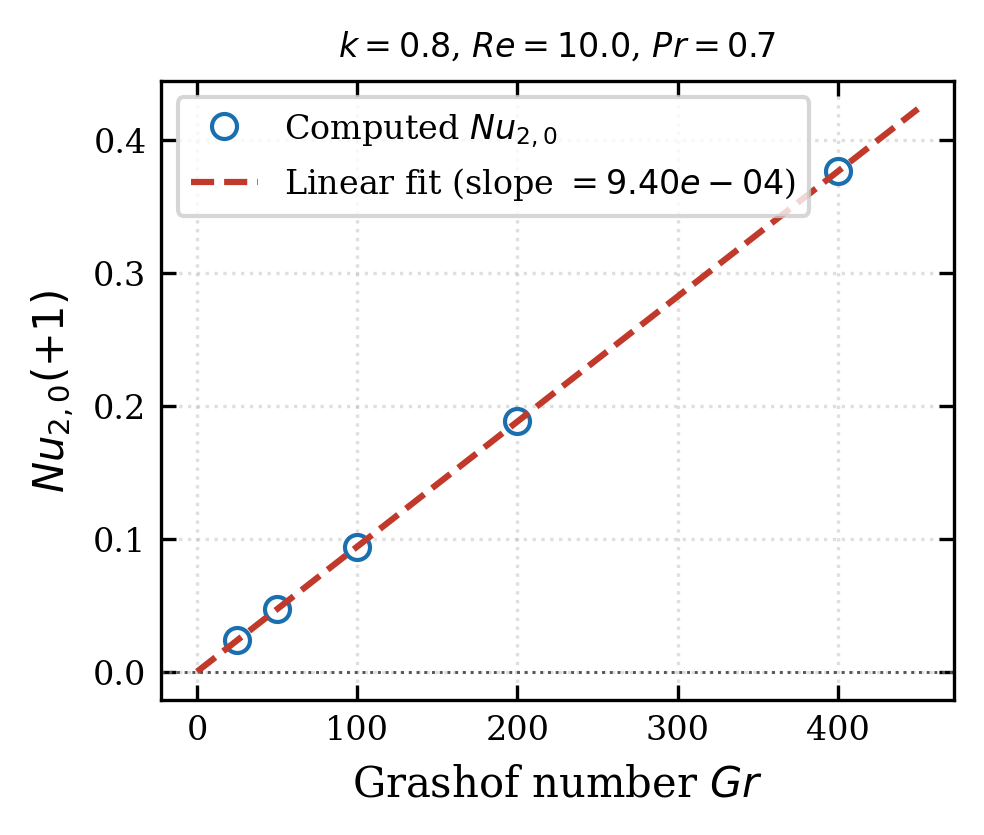
\includegraphics[width=0.55\textwidth]{fig05_Gr_sweep.png}
  \caption{Thermal pumping coefficient versus Grashof number at fixed $(k,\Rey,\Pr)=(0.8,10,0.7)$.
  The free-intercept fit is effectively exact and the response vanishes in the forced-convection limit
  $\Grr=0$.}
  \label{fig:Gr_sweep}
\end{figure}
\begin{figure}[htb]
  \centering
  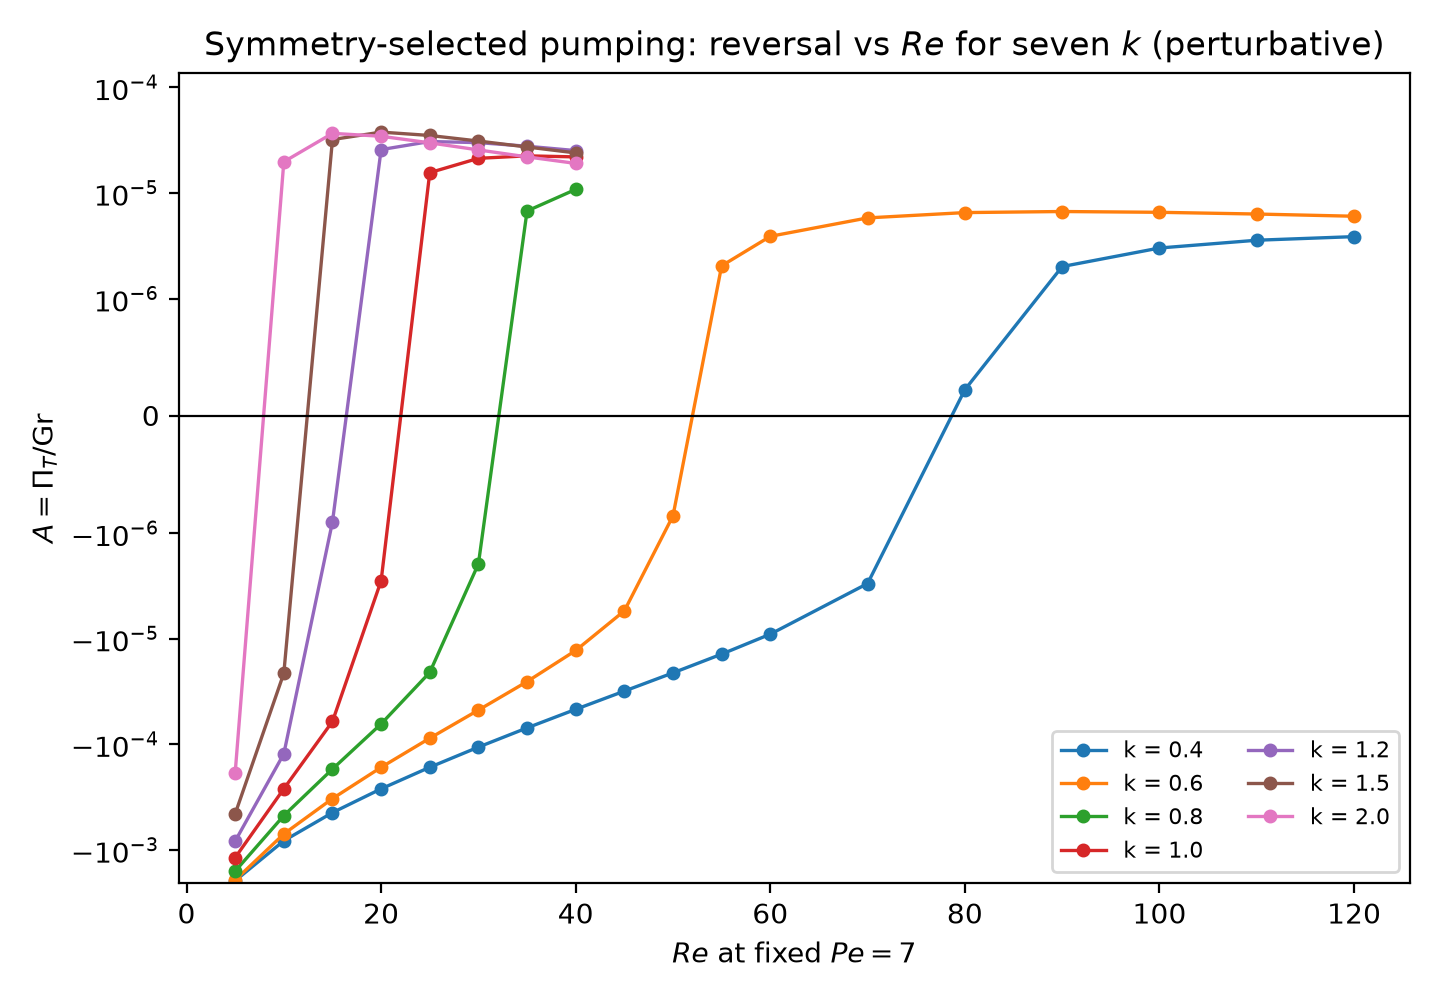
\includegraphics[width=0.72\textwidth]{campaign_v2_symmetry_selection/FIG_v2_01_piT_vs_Re_kartsch.png}
  \caption{Normalized pumping response $A=\PiT/\Grr$ versus Reynolds number at fixed
  $\Pe=7$ and $\Grr=100$ for seven wavenumbers, computed with the authoritative
  perturbative solver. Each curve crosses zero exactly once. The $k=0.4$ and
  $k=0.6$ curves are drawn over the extended interval $\Rey\le120$ that their
  crossings require; the remaining five use the primary $\Rey\le40$ window,
  inside which each of them already crosses. The crossing moves to lower
  $\Rey$ as $k$ increases.}
  \label{fig:Rec_kartsch}
\end{figure}
\begin{figure}[htb]
  \centering
  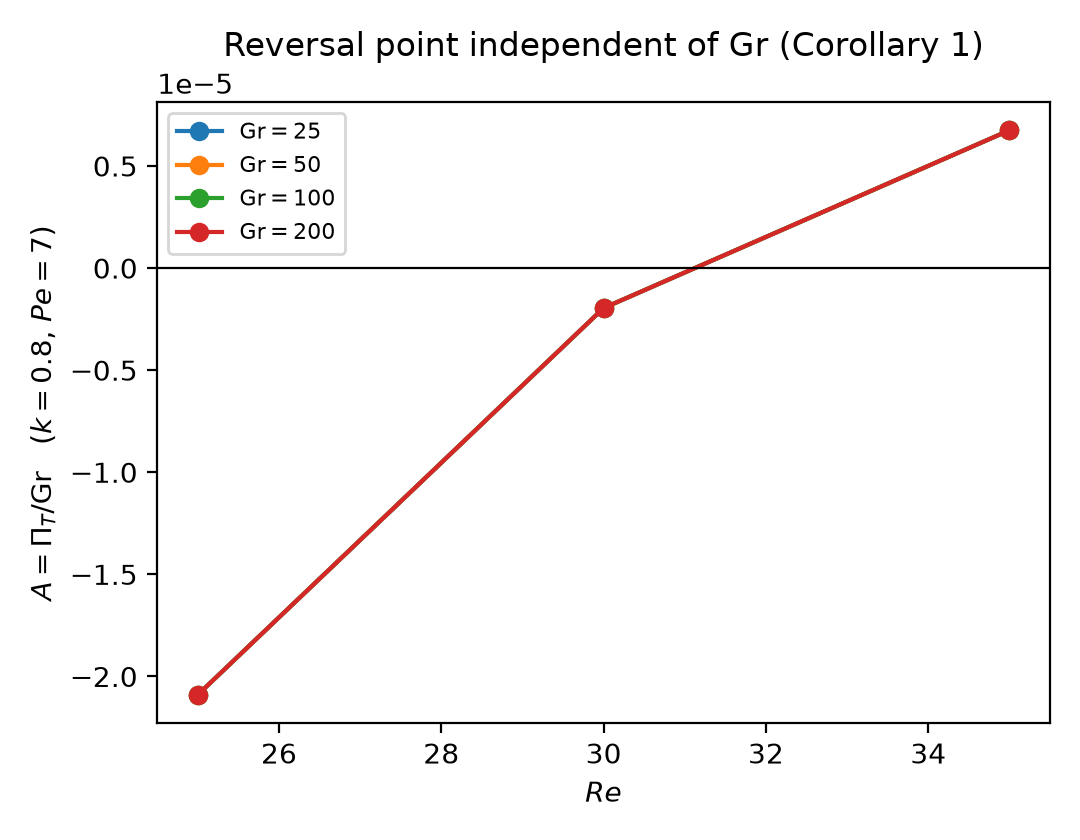
\includegraphics[width=0.58\textwidth]{campaign_v2_symmetry_selection/FIG_v2_03_Gr_invariance.png}
  \caption{Normalized response $A=\PiT/\Grr$ versus $\Rey$ at $k=0.8$ and $\Pe=7$ for
  four Grashof numbers. The four curves coincide, as required by
  Corollary~\ref{cor:Gr_independence}.}
  \label{fig:Gr_invariance}
\end{figure}
\begin{table}[htb]
  \centering
  \caption{Test of Corollary~\ref{cor:Gr_independence} at $k=0.8$, $\Pe=7$. The
  normalized response is invariant to a worst-case relative spread of
  $7.3\times10^{-11}$ and the reversal
  Reynolds number is identical to the nine displayed digits for all four Grashof
  numbers (absolute spread $1.2\times10^{-10}$); the scan is archived as
  group B of the data package.}
  \label{tab:Gr_invariance}
  \begin{ruledtabular}
  \begin{tabular}{c|rrr|c}
  $\Grr$ & $A(\Rey=25)$ & $A(\Rey=30)$ & $A(\Rey=35)$ & $\Rey_c$ \\ \hline
  25   & $-2.089882\times10^{-5}$ & $-1.958845\times10^{-6}$ & $+6.745165\times10^{-6}$ & 30.838496520 \\
  50   & $-2.089882\times10^{-5}$ & $-1.958845\times10^{-6}$ & $+6.745165\times10^{-6}$ & 30.838496520 \\
  100  & $-2.089882\times10^{-5}$ & $-1.958845\times10^{-6}$ & $+6.745165\times10^{-6}$ & 30.838496520 \\
  200  & $-2.089882\times10^{-5}$ & $-1.958845\times10^{-6}$ & $+6.745165\times10^{-6}$ & 30.838496520 \\
  \end{tabular}
  \end{ruledtabular}
\end{table}

\section{Verification of the nonlinear DNS}
\begin{figure}[htb]
\centering
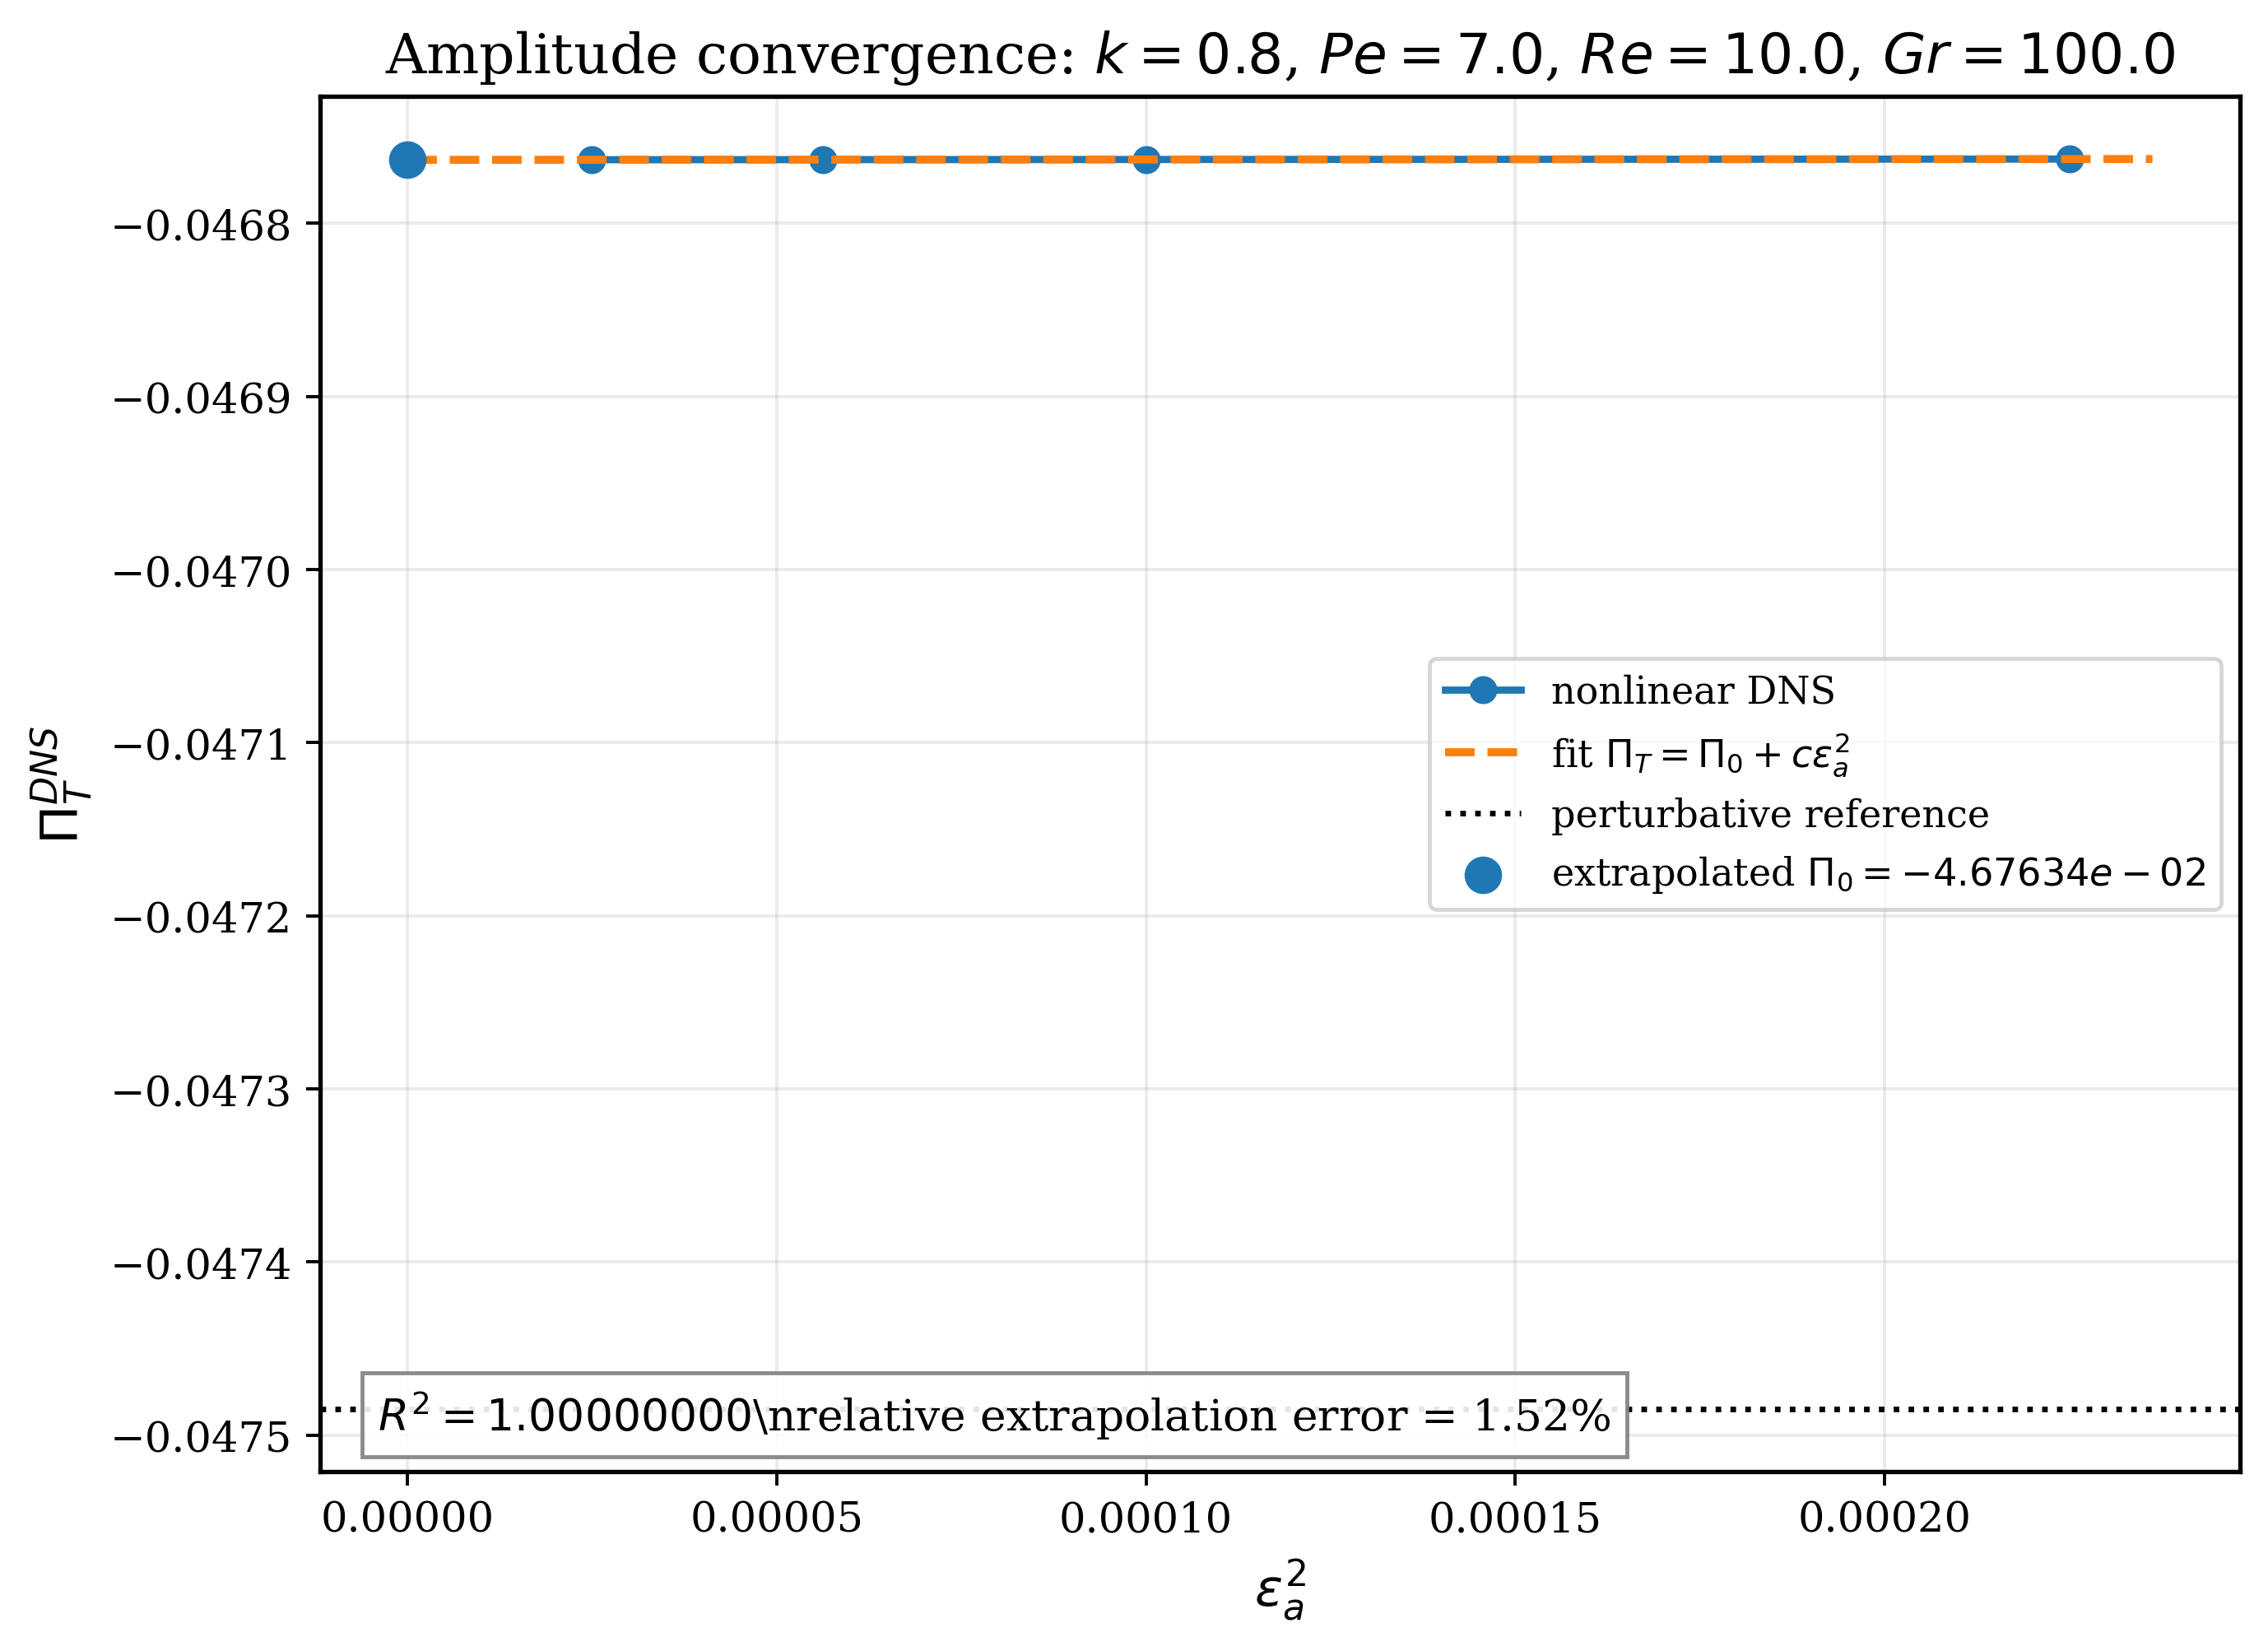
\includegraphics[width=0.76\textwidth]
{FIG01_dns_amplitude_convergence.png}
\caption{
Convergence of the fully nonlinear DNS pumping coefficient with decreasing
asymmetry amplitude. The nonlinear DNS values approach a finite
$\varepsilon_a\rightarrow0$ limit, which differs by only $1.52\%$ from the
second-order perturbative prediction. The result provides an independent
nonlinear validation of the asymptotic pumping coefficient.
}
\label{fig:dns_amplitude}
\end{figure}
\begin{figure}[htb]
\centering
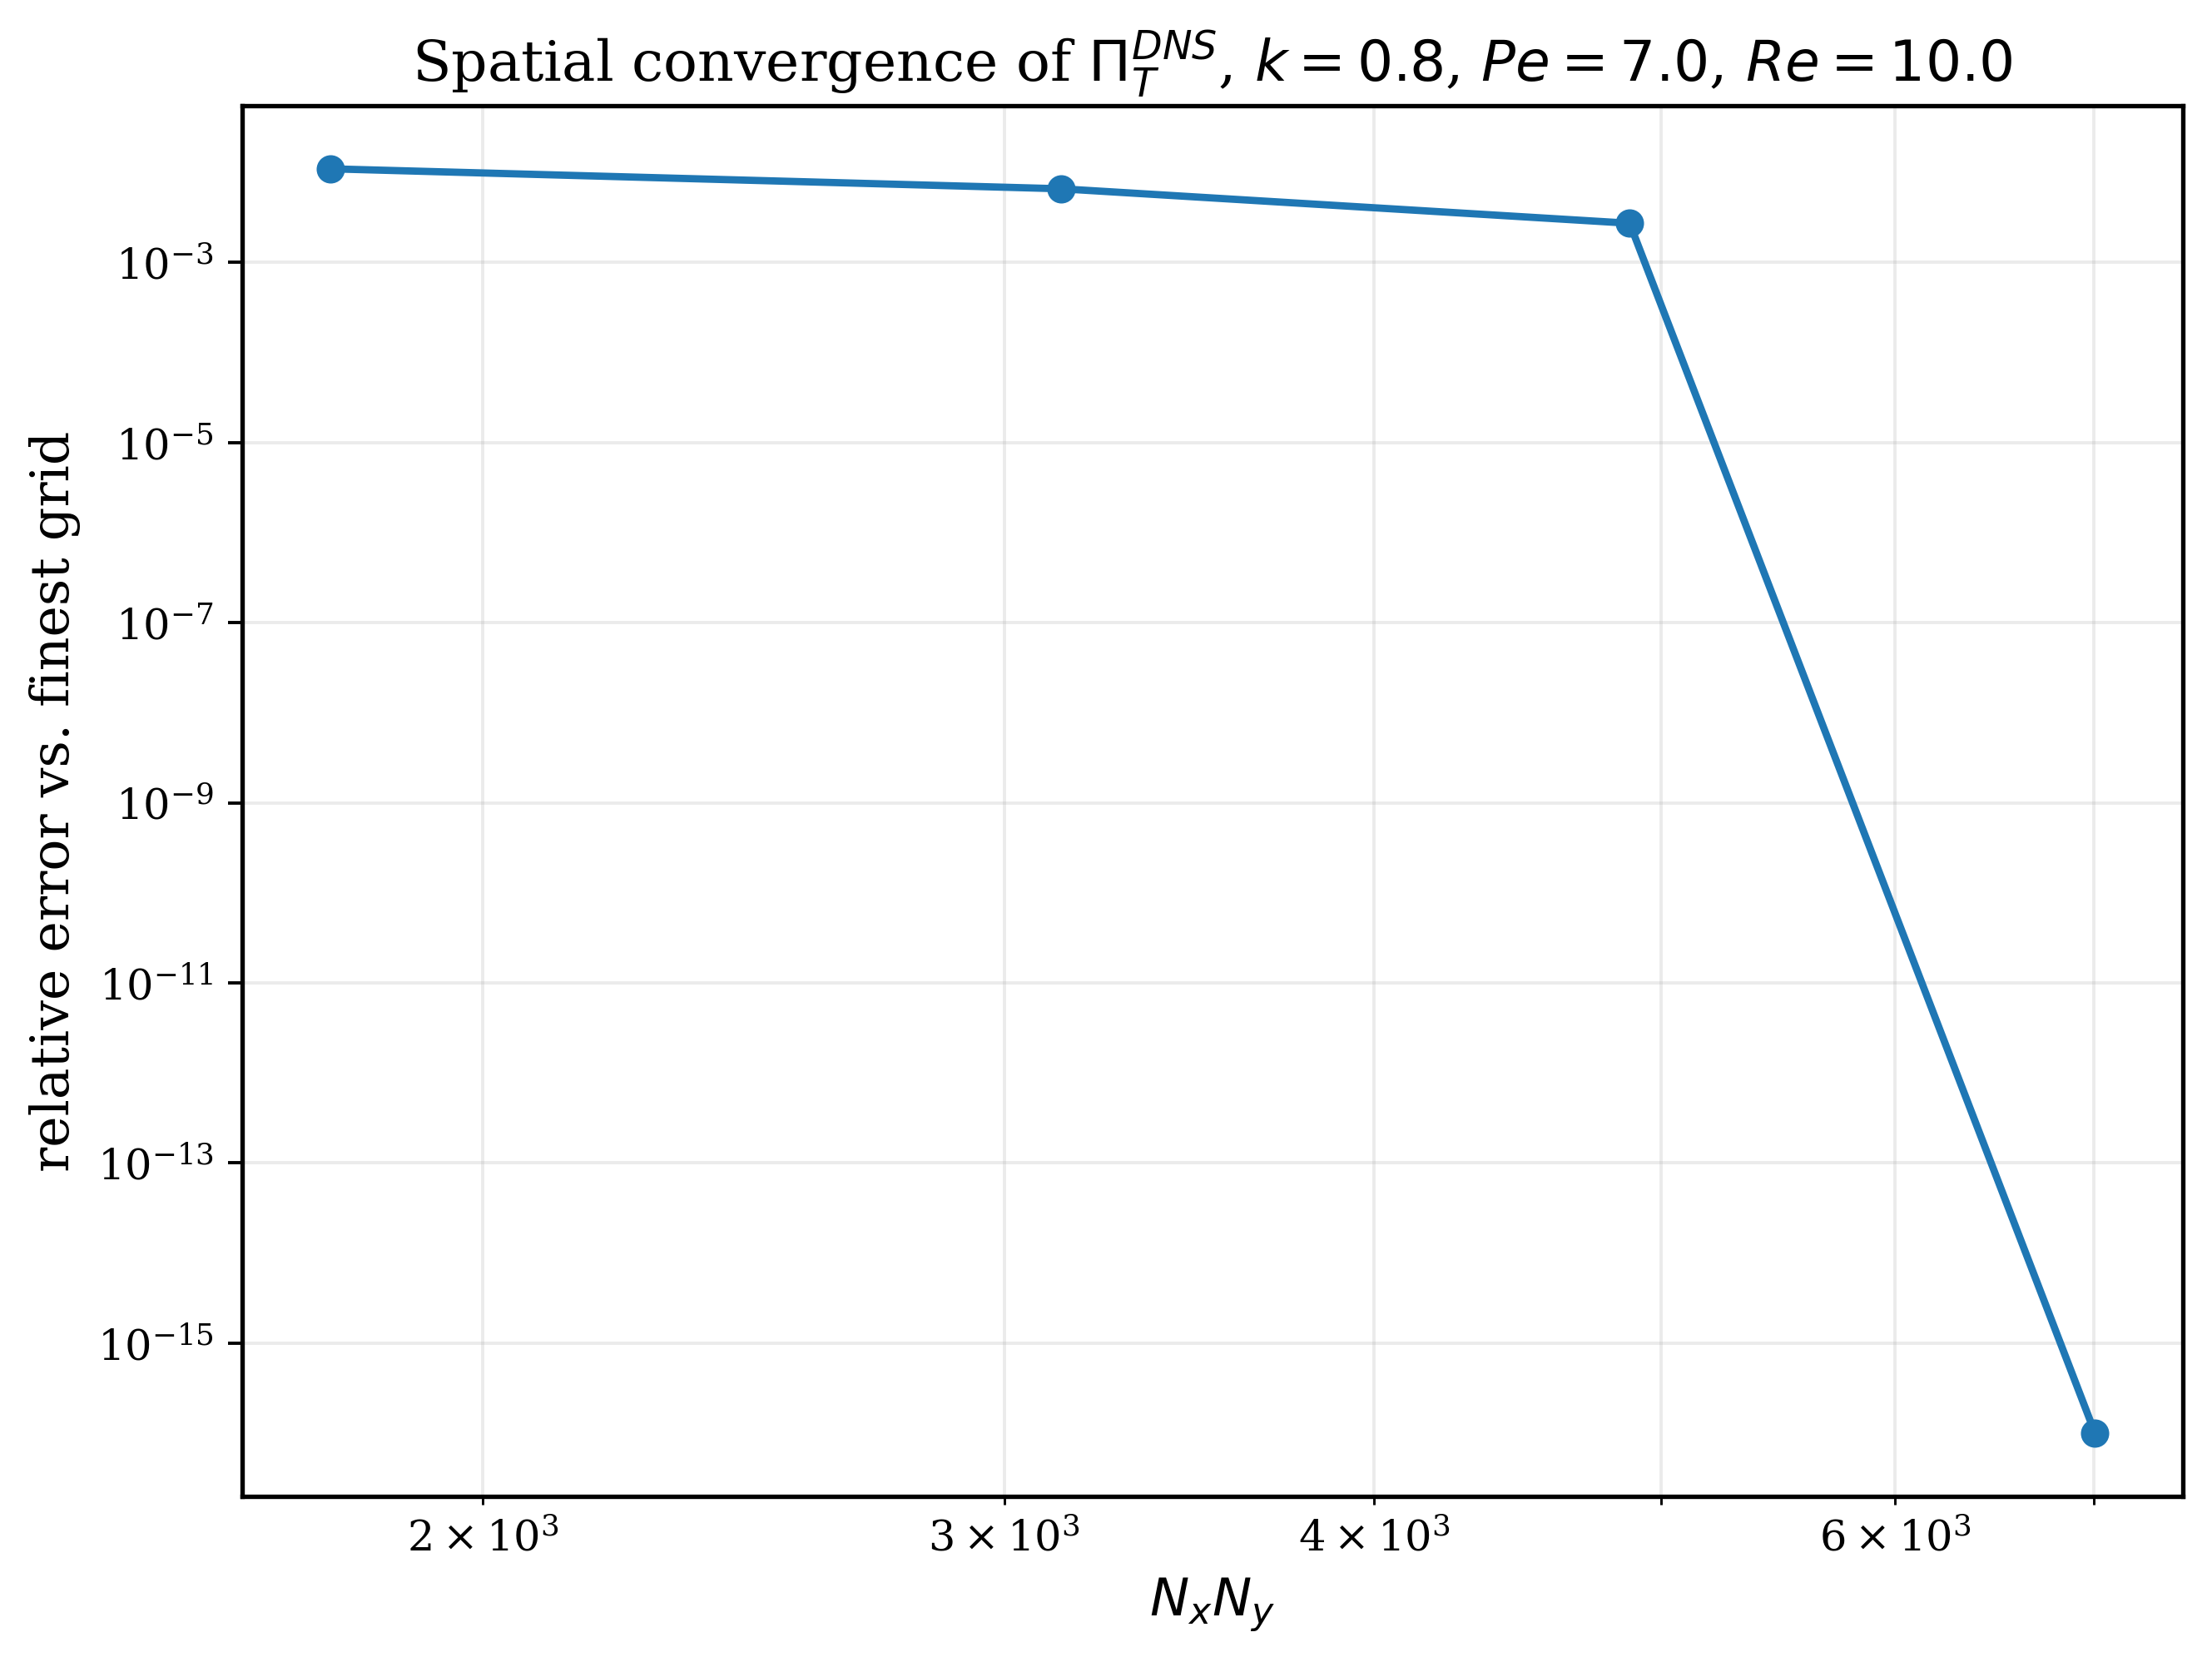
\includegraphics[width=0.76\textwidth]
{FIG02_dns_spatial_convergence.png}
\caption{
Spatial convergence of the nonlinear DNS pumping coefficient. The solution
approaches a well-defined finest-grid value as both the streamwise and
transverse resolutions are increased. The remaining difference between the
finest-grid DNS result and the perturbative reference is smaller than the
total discrepancy observed on coarser meshes.
}
\label{fig:dns_spatial}
\end{figure}
\begin{figure}[htb]
\centering
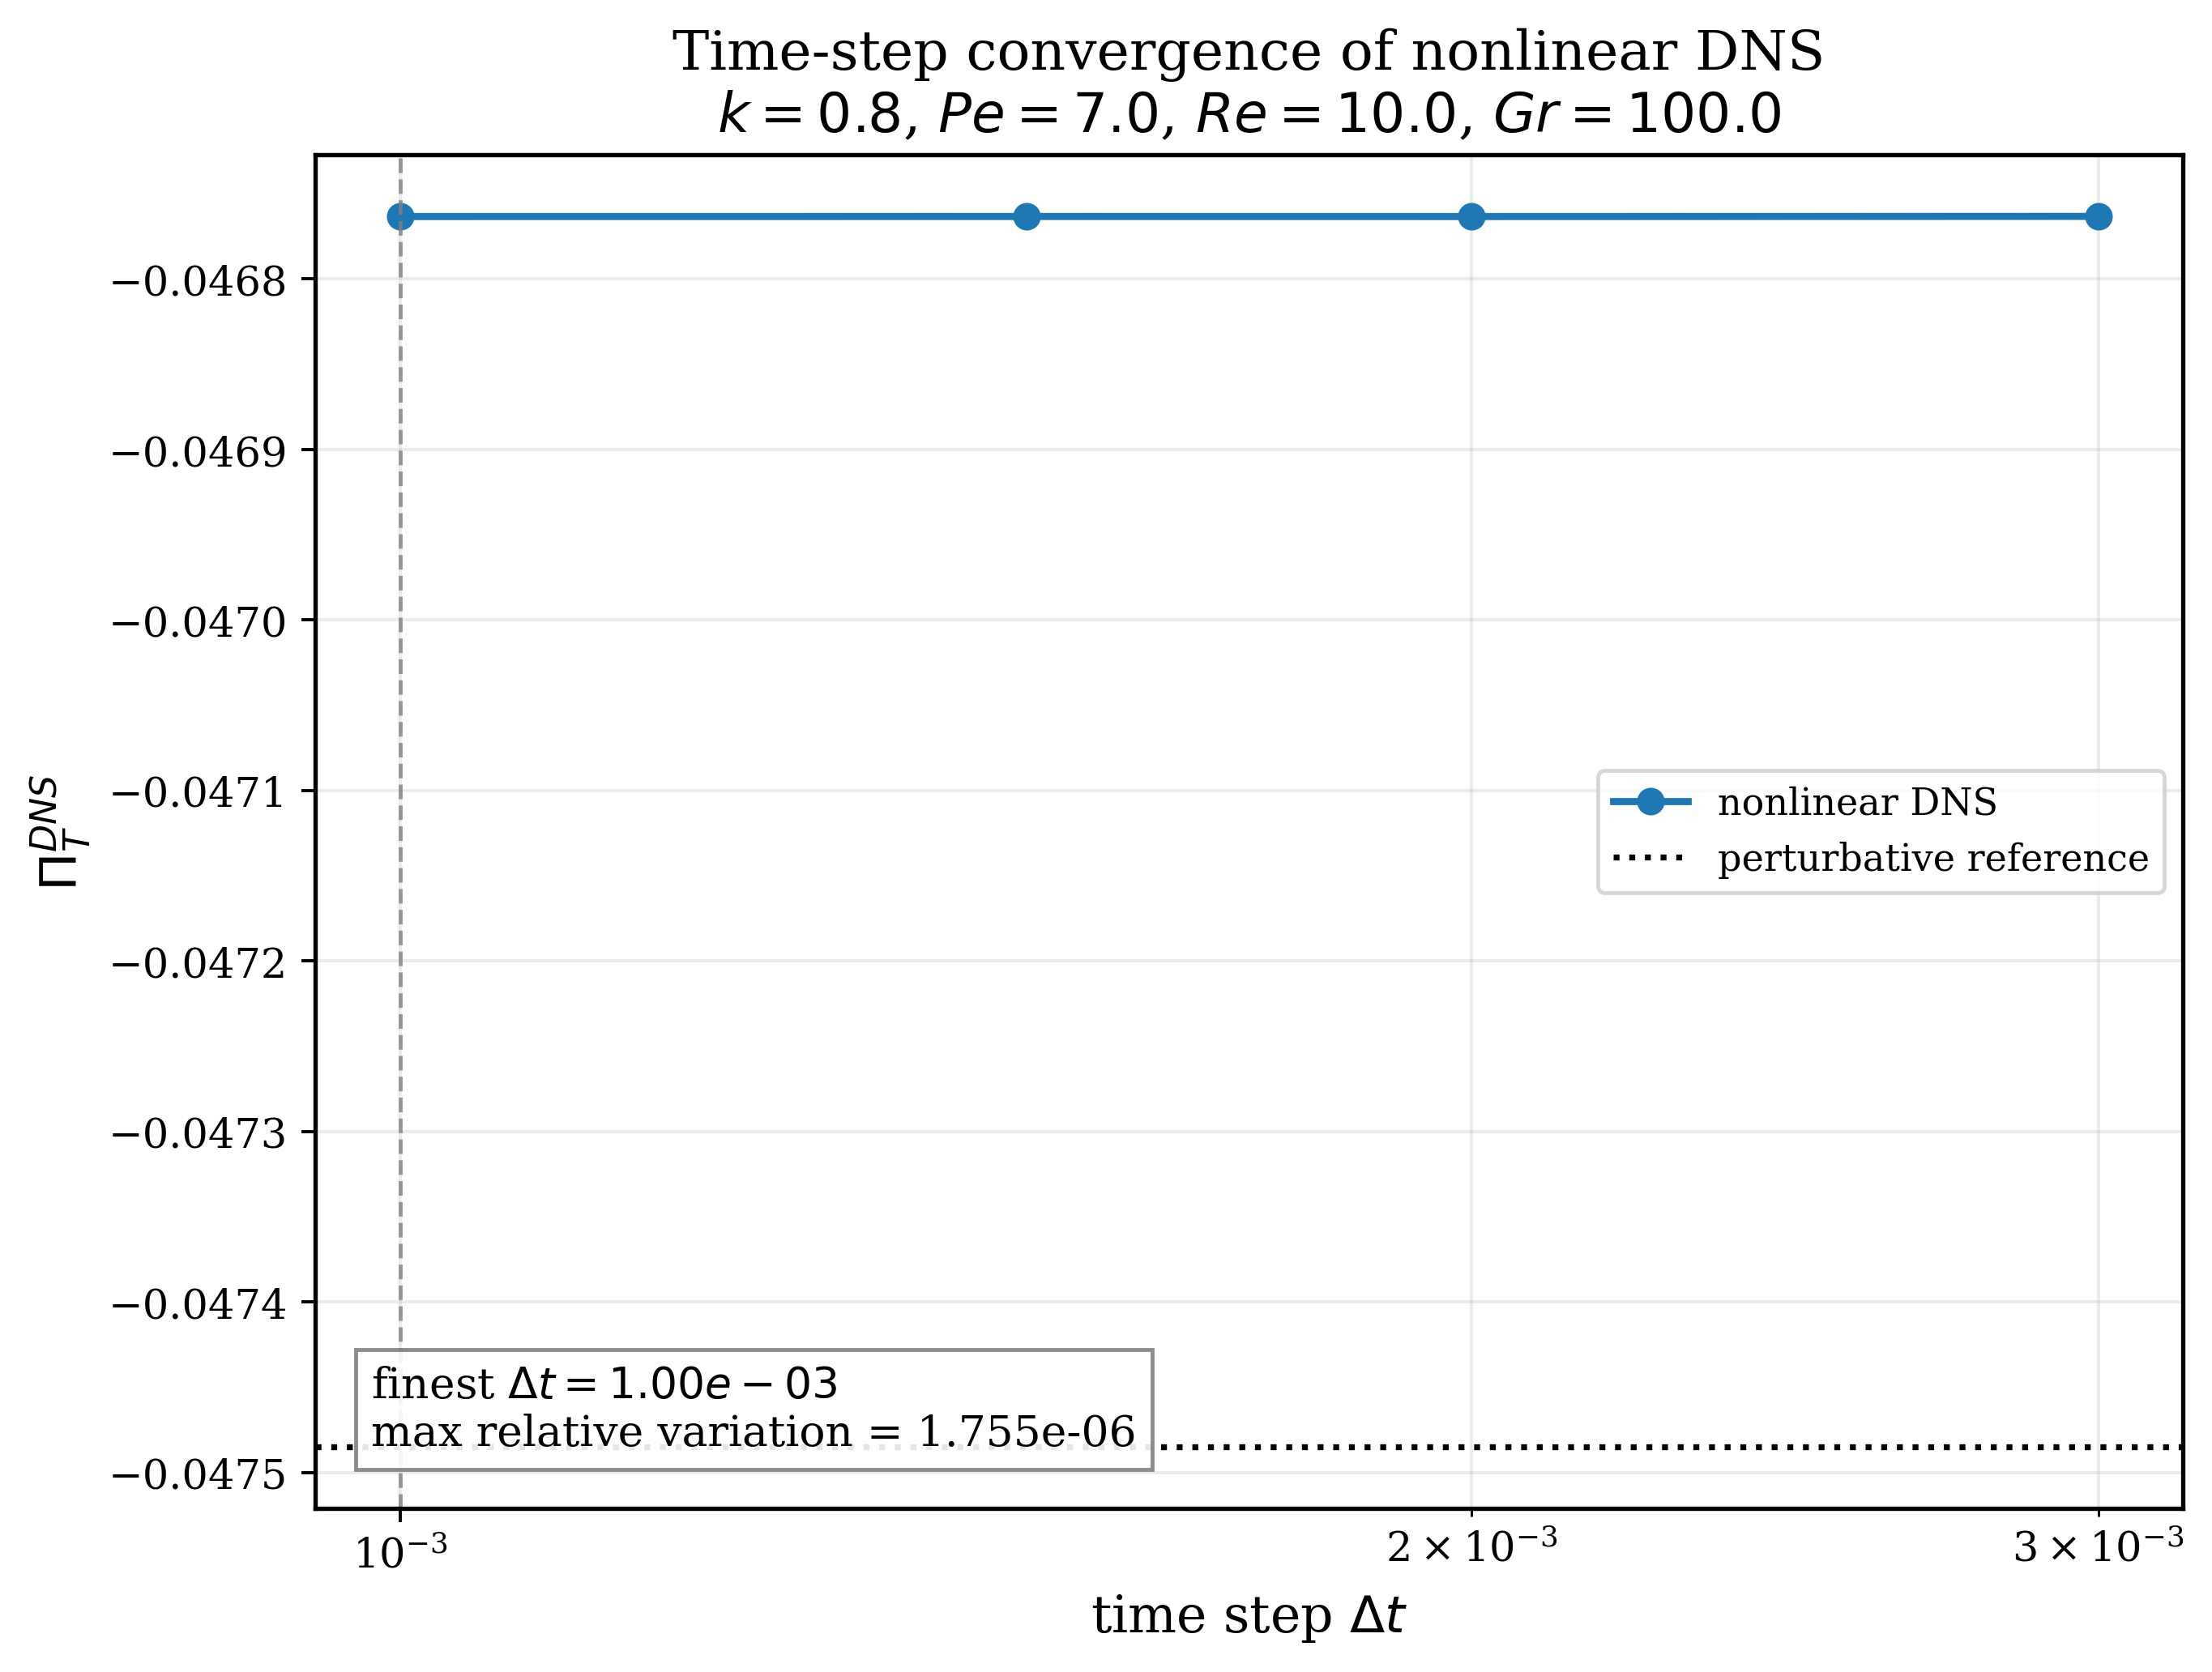
\includegraphics[width=0.76\textwidth]
{FIG03_dns_timestep_convergence.png}
\caption{
Time-step convergence of the nonlinear DNS pumping coefficient. The response
remains unchanged to within approximately $10^{-6}$ in relative terms over
the tested time-step range, confirming that the stationary wall-flux
observable is temporally converged.
}
\label{fig:dns_timestep}
\end{figure}
\begin{figure}[htb]
\centering
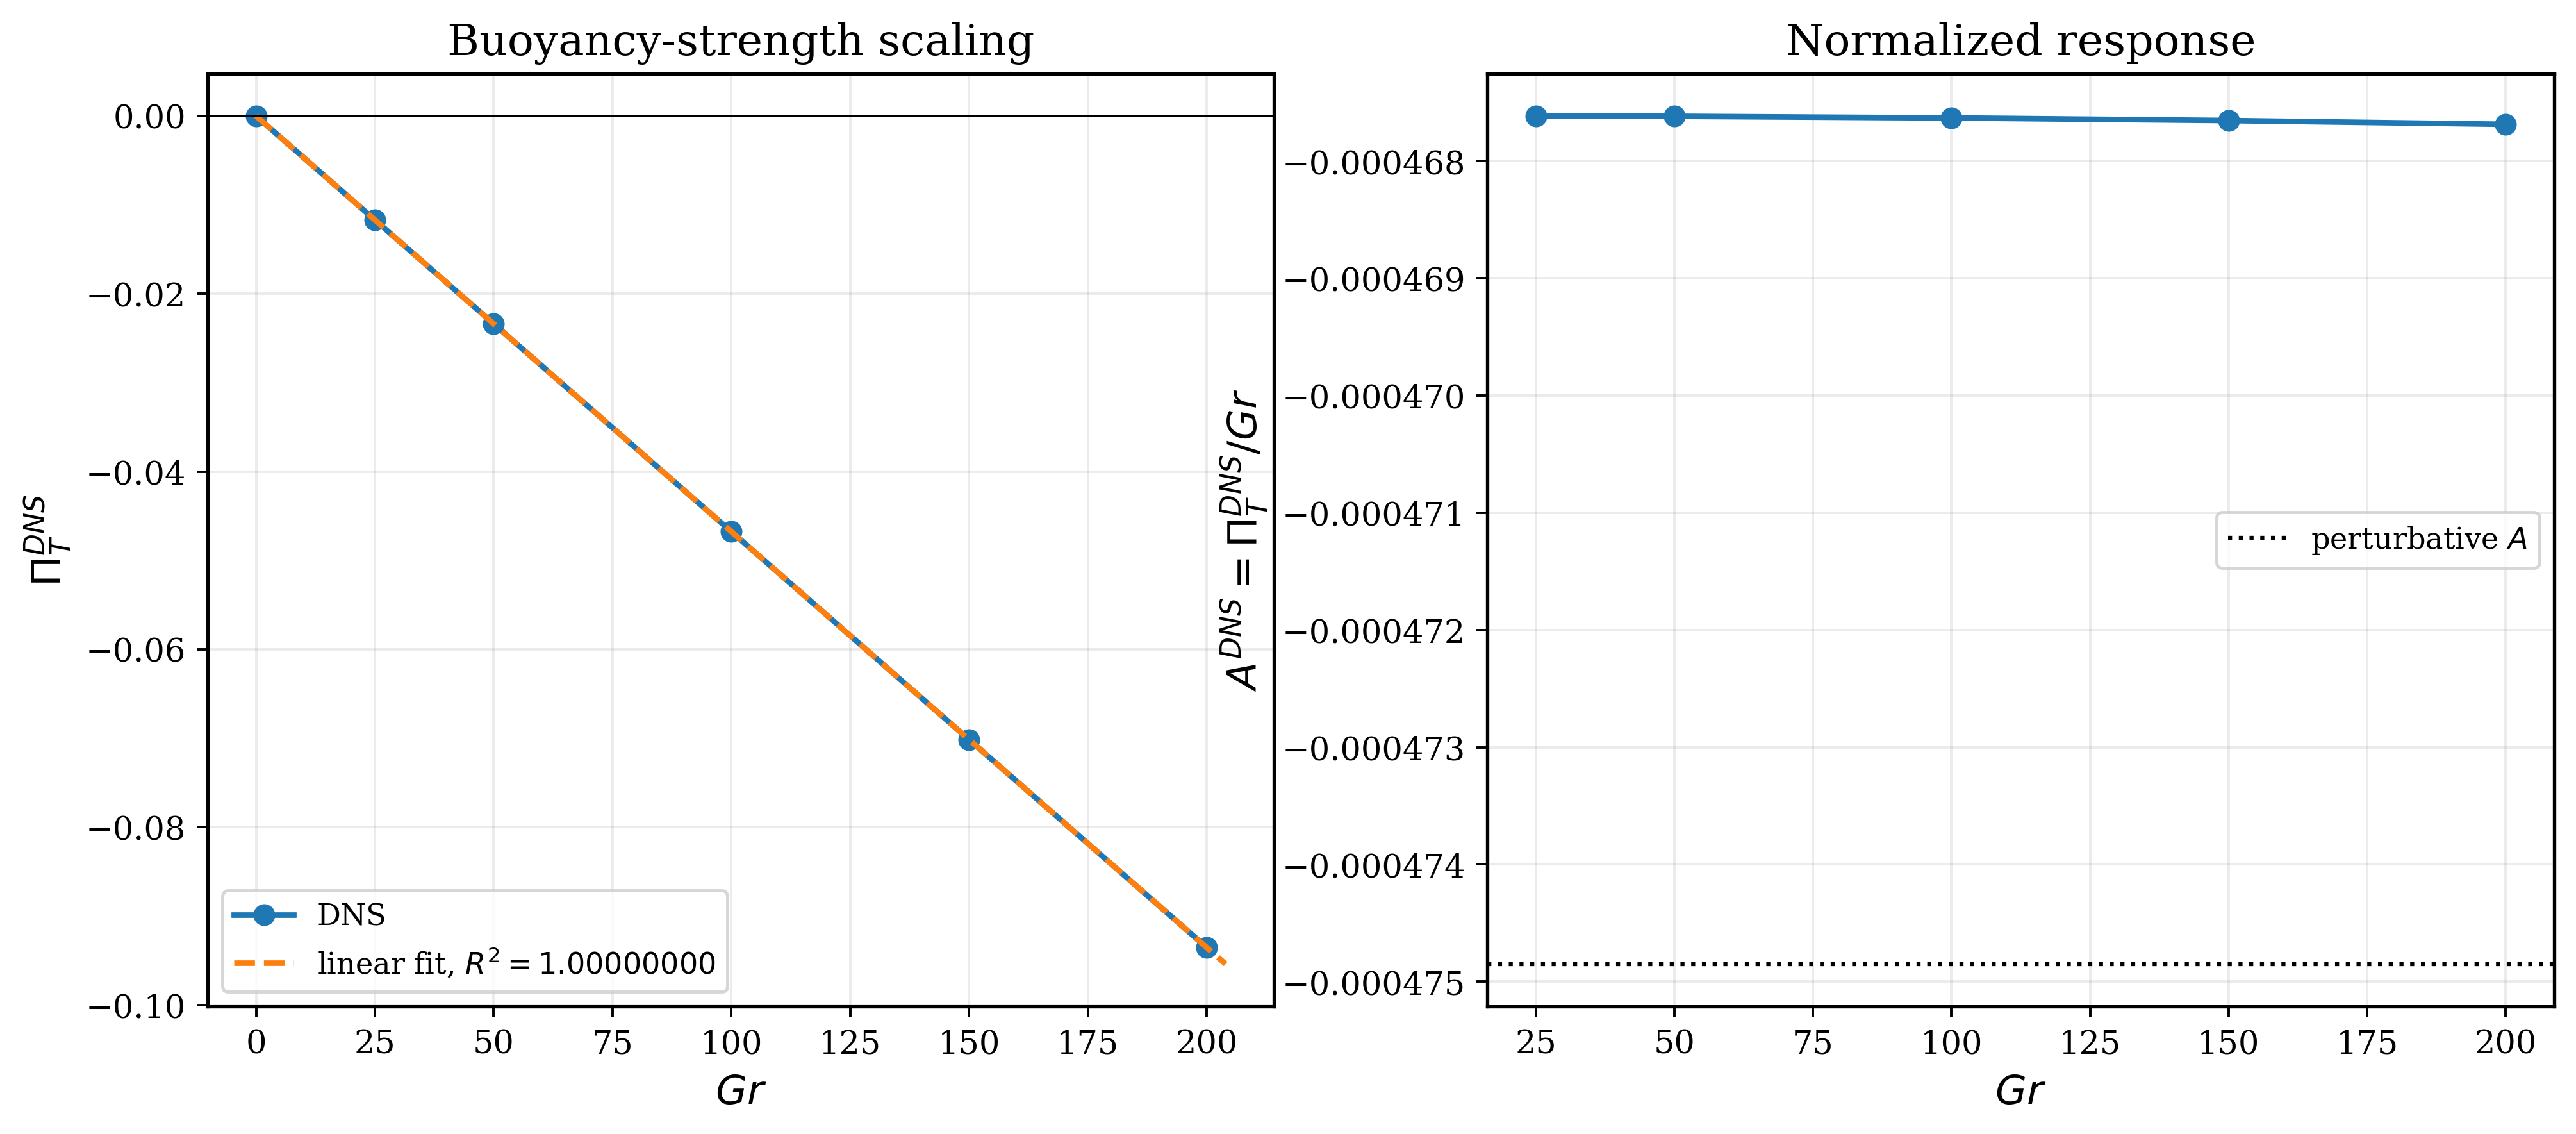
\includegraphics[width=0.78\textwidth]
{FIG04_dns_gr_scaling.png}
\caption{
Nonlinear DNS verification of the Grashof-number scaling at fixed
$(k,\Rey,\Pr)=(0.8,10,0.7)$. The pumping coefficient is linear in $\Grr$
over the investigated interval, while the $\Grr=0$ calculation switches off
the leading pumping response to numerical precision. The result independently
confirms the analytical proportionality $\PiT=\Grr A(k,\Rey,\Pr)$.
}
\label{fig:dns_gr}
\end{figure}
\begin{figure}[htb]
\centering
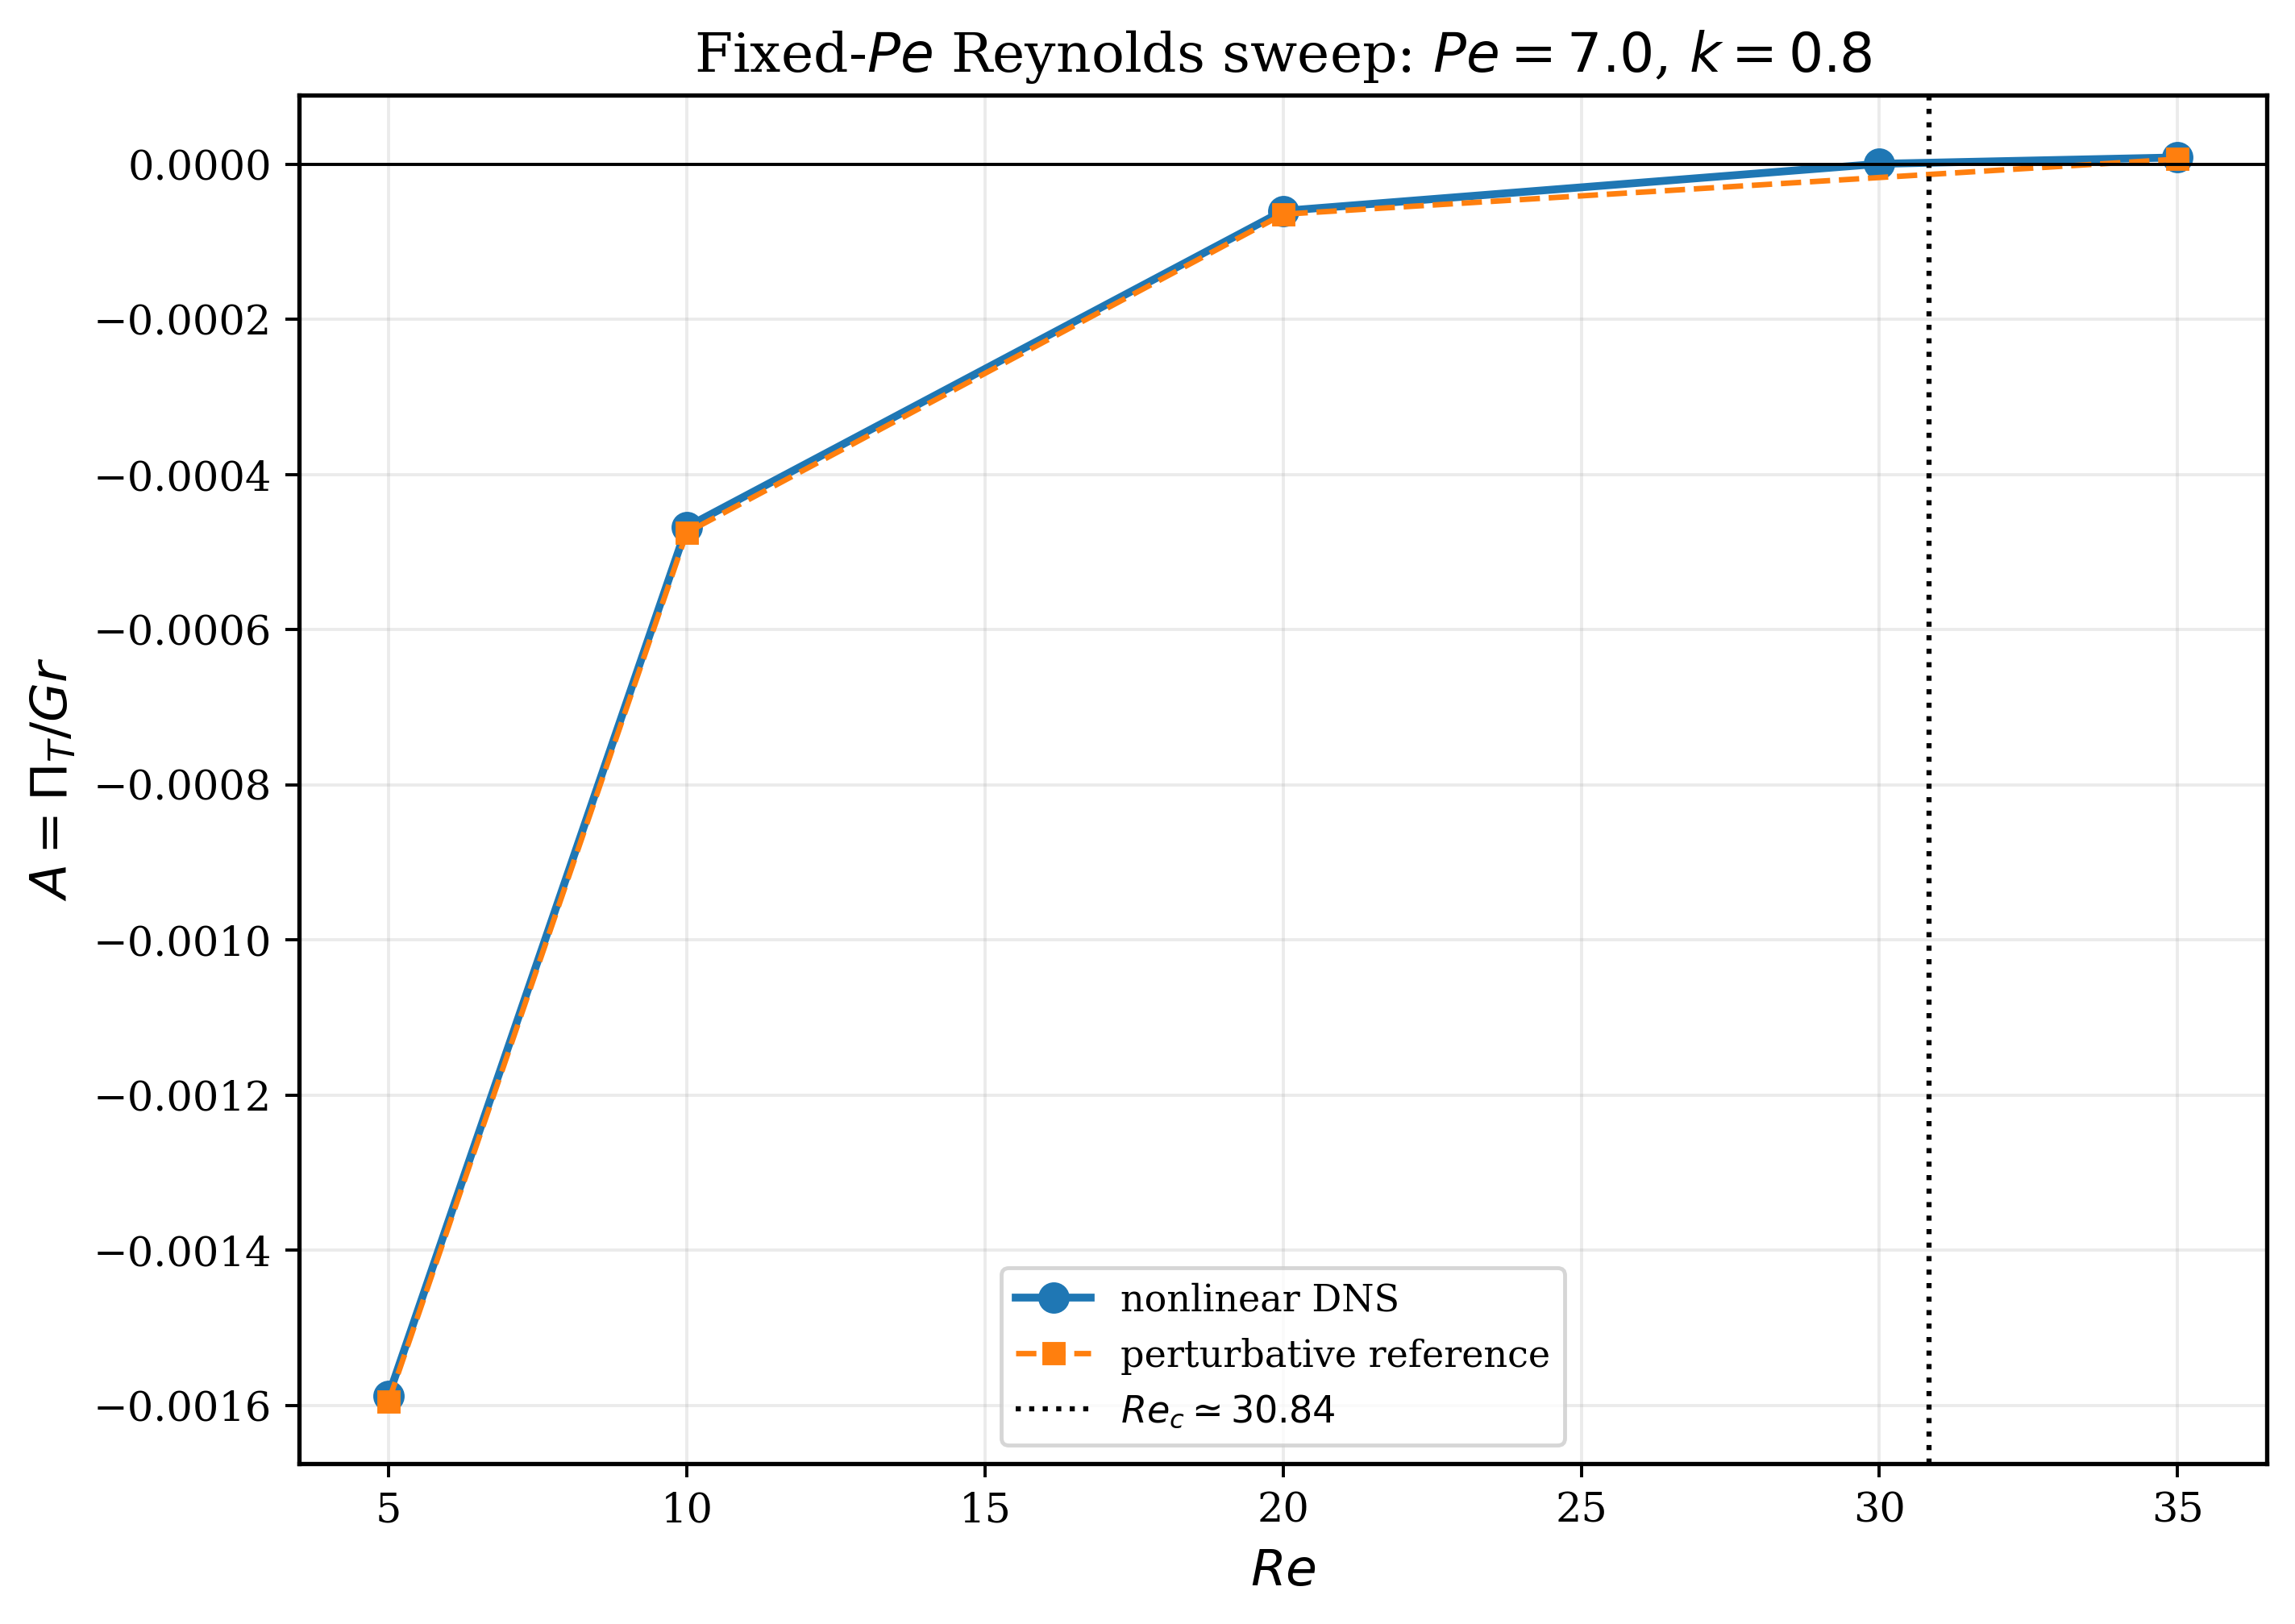
\includegraphics[width=0.78\textwidth]
{FIG05_dns_re_dependence.png}
\caption{
Normalized pumping response $A=\PiT/\Grr$ from the independent nonlinear DNS
at fixed $\Pe=7$, $k=0.8$, and $\Grr=100$. Varying $\Rey$ changes both the magnitude
and the sign of the response. The transition from negative values at
$\Rey=20$ to positive values at $\Rey=30$ and $35$ provides direct nonlinear
evidence that the hydrodynamic Reynolds number remains an active control
parameter even when the P\'eclet number is held fixed.
}
\label{fig:dns_re}
\end{figure}
\begin{table}[htb]
\centering
\caption{
Independent nonlinear DNS at fixed $\Pe=7$, $k=0.8$, and $\Grr=100$.
The Prandtl number is adjusted according to $\Pr=\Pe/\Rey$.
}
\label{tab:dns_re_sweep}
\begin{ruledtabular}
\begin{tabular}{ccccc}
$\Rey$ & $\Pr$ & $A_{\mathrm{DNS}}$ & $A_{\mathrm{pert}}$ & Relative difference \\
\hline
5
& 1.4000
& $-1.5878\times10^{-3}$
& $-1.5951\times10^{-3}$
& $0.46\%$ \\
10
& 0.7000
& $-4.6763\times10^{-4}$
& $-4.7485\times10^{-4}$
& $1.52\%$ \\
20
& 0.3500
& $-5.9977\times10^{-5}$
& $-6.4279\times10^{-5}$
& $6.69\%$ \\
30
& 0.2333
& $+7.5042\times10^{-7}$
& --
& -- \\
35
& 0.2000
& $+8.9842\times10^{-6}$
& $+6.7452\times10^{-6}$
& $33.19\%$ \\
\end{tabular}
\end{ruledtabular}
\end{table}

\section{Phase decomposition, term balance and transport comparison}
\begin{figure}[htb]
  \centering
  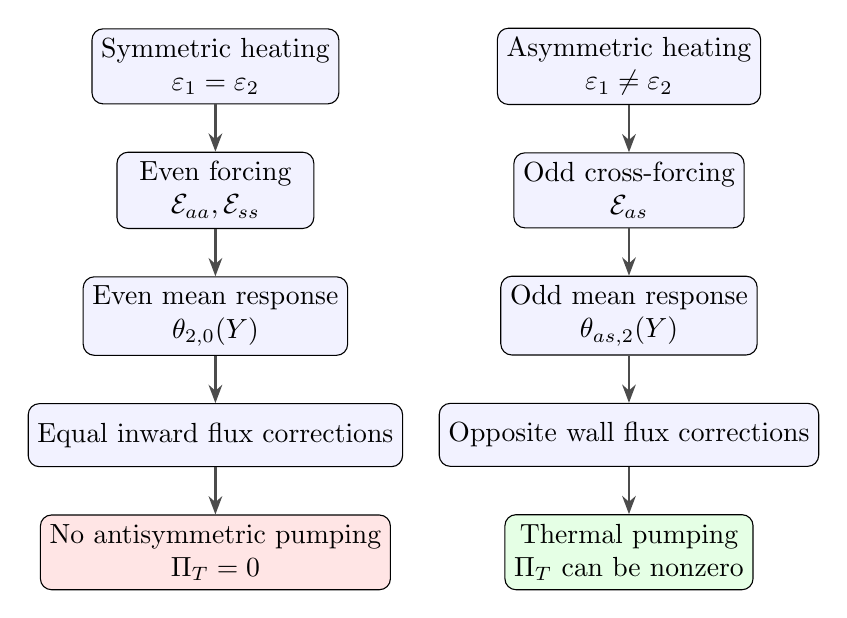
\begin{tikzpicture}[
      node distance=1.5cm and 2cm,
      box/.style={draw, rectangle, rounded corners, minimum width=2.5cm, minimum height=0.8cm, align=center, fill=blue!5},
      arrow/.style={-Stealth, thick, color=black!70}
    ]
    \node[box] (sym1) {Symmetric heating\\$\varepsilon_1 = \varepsilon_2$};
    \node[box, below=0.6cm of sym1] (sym2) {Even forcing\\$\mathcal{E}_{aa},\mathcal{E}_{ss}$};
    \node[box, below=0.6cm of sym2] (sym3) {Even mean response\\$\theta_{2,0}(Y)$};
    \node[box, below=0.6cm of sym3] (sym4) {Equal inward flux corrections};
    \node[box, fill=red!10, below=0.6cm of sym4] (sym5) {No antisymmetric pumping\\$\PiT=0$};

    \node[box, right=2cm of sym1] (asym1) {Asymmetric heating\\$\varepsilon_1\neq\varepsilon_2$};
    \node[box, below=0.6cm of asym1] (asym2) {Odd cross-forcing\\$\mathcal{E}_{as}$};
    \node[box, below=0.6cm of asym2] (asym3) {Odd mean response\\$\theta_{as,2}(Y)$};
    \node[box, below=0.6cm of asym3] (asym4) {Opposite wall flux corrections};
    \node[box, fill=green!10, below=0.6cm of asym4] (asym5) {Thermal pumping\\$\PiT$ can be nonzero};

    \draw[arrow] (sym1) -- (sym2);
    \draw[arrow] (sym2) -- (sym3);
    \draw[arrow] (sym3) -- (sym4);
    \draw[arrow] (sym4) -- (sym5);
    \draw[arrow] (asym1) -- (asym2);
    \draw[arrow] (asym2) -- (asym3);
    \draw[arrow] (asym3) -- (asym4);
    \draw[arrow] (asym4) -- (asym5);
  \end{tikzpicture}
  \caption{Logical chain connecting wall-temperature symmetry to the nonlinear wall-flux response.}
  \label{fig:logic_diagram}
\end{figure}
\begin{figure}[htb]
  \centering
  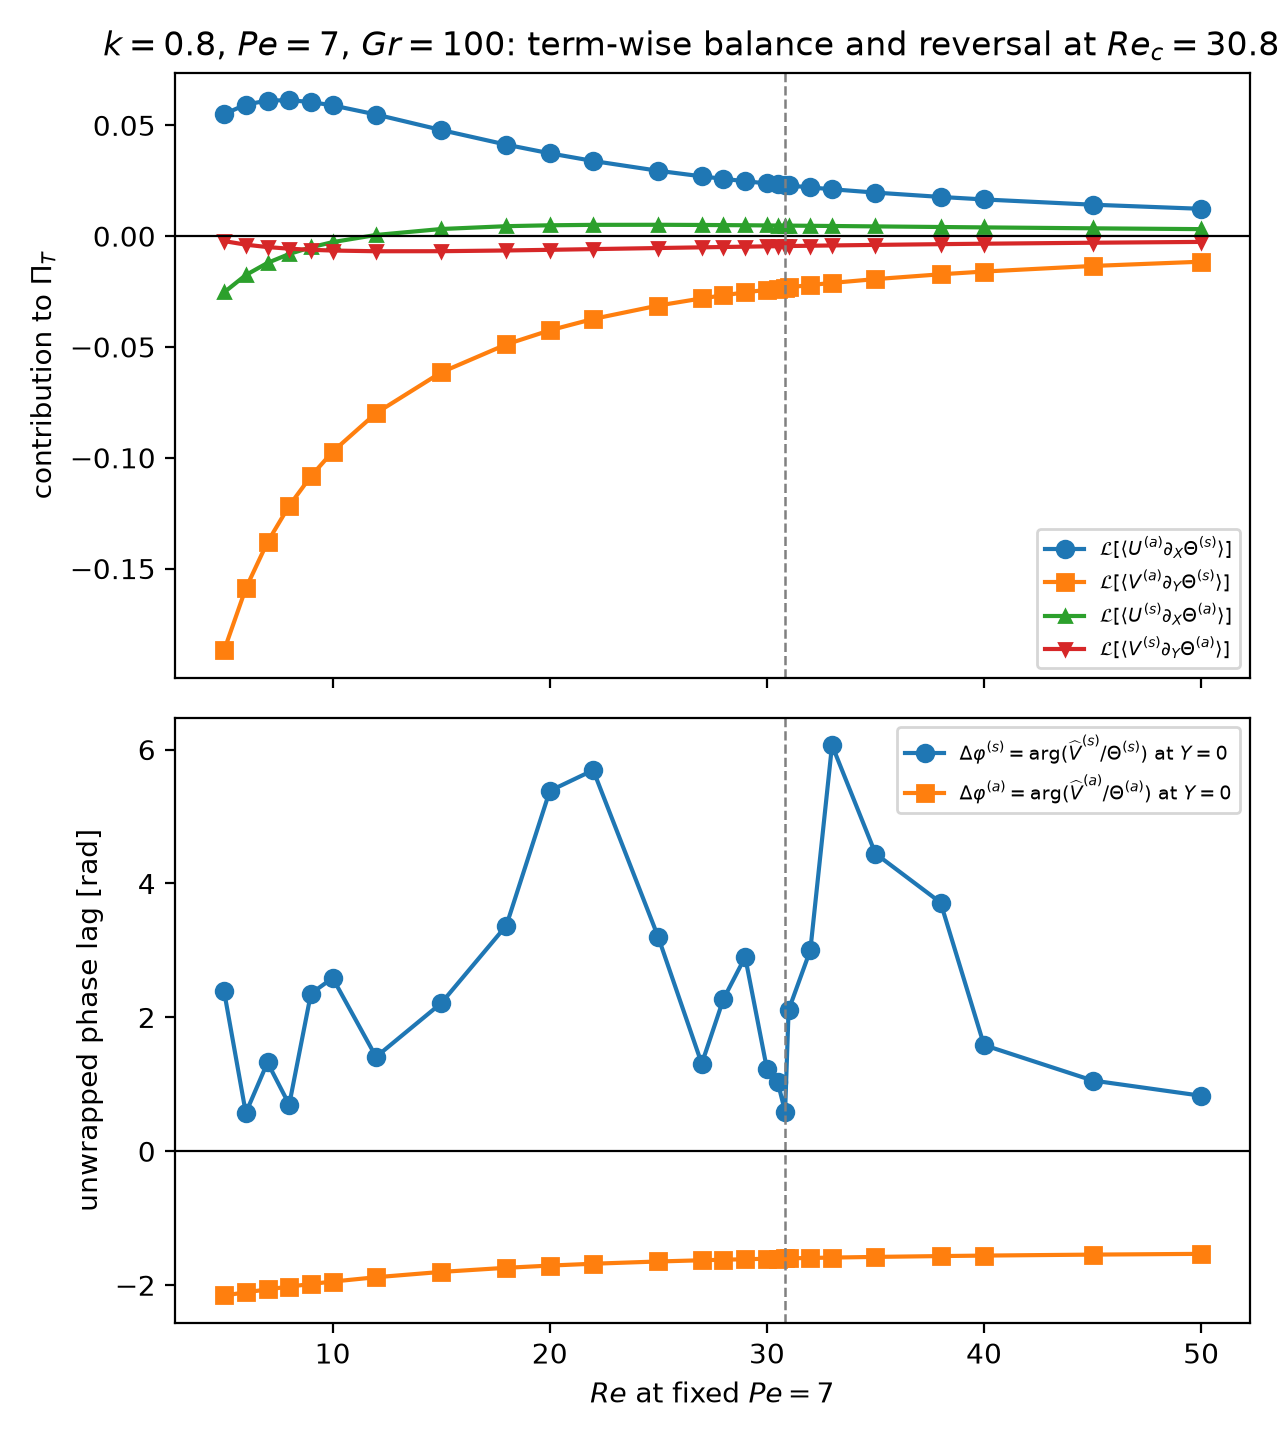
\includegraphics[width=0.72\textwidth]{campaign_v2_symmetry_selection/FIG_v2_08_phase_crossing.png}
  \caption{Upper panel: the four additive contributions \eqref{eq:term_decomp} to
  $\PiT$ versus $\Rey$ at $k=0.8$, $\Pe=7$; the dashed line marks
  $\Rey_c=30.838$. Lower panel: unwrapped centreline phase lags, which vary smoothly
  and cross zero nowhere, showing that the reversal is a balance effect rather than a
  phase-sign effect.}
  \label{fig:phase_crossing}
\end{figure}
\begin{table}[htb]
  \centering
  \caption{Term-wise balance of $\PiT$ at $k=0.8$, $\Pe=7$, $\Grr=100$ with
  $\Pr=\Pe/\Rey$. The two dominant contributions keep fixed signs---the streamwise
  advection term is positive, the wall-normal sweep term negative---and the reversal
  occurs when the faster decay of the sweep term lets the two cancel; the
  term-by-term evaluation is archived as group B of the data package.}
  \label{tab:term_balance}
  \begin{ruledtabular}
  \scriptsize
  \setlength{\tabcolsep}{4pt}
  \begin{tabular}{@{\hspace{3pt}}r|rrrr|r@{\hspace{3pt}}}
  $\Rey$ & $\mathcal L[\langle U^{(a)}\partial_X\Theta^{(s)}\rangle]$
         & $\mathcal L[\langle V^{(a)}\partial_Y\Theta^{(s)}\rangle]$
         & $\mathcal L[\langle U^{(s)}\partial_X\Theta^{(a)}\rangle]$
         & $\mathcal L[\langle V^{(s)}\partial_Y\Theta^{(a)}\rangle]$
         & $\PiT$ \\ \hline
  5  &  $5.504\times10^{-2}$ & $-1.870\times10^{-1}$ & $-2.537\times10^{-2}$ & $-2.236\times10^{-3}$ & $-1.595\times10^{-1}$ \\
  10 &  $5.899\times10^{-2}$ & $-9.726\times10^{-2}$ & $-2.707\times10^{-3}$ & $-6.504\times10^{-3}$ & $-4.749\times10^{-2}$ \\
  20 &  $3.737\times10^{-2}$ & $-4.251\times10^{-2}$ & $+4.895\times10^{-3}$ & $-6.180\times10^{-3}$ & $-6.428\times10^{-3}$ \\
  30 &  $2.378\times10^{-2}$ & $-2.420\times10^{-2}$ & $+4.829\times10^{-3}$ & $-4.611\times10^{-3}$ & $-1.959\times10^{-4}$ \\
  $\Rey_c$ & $2.300\times10^{-2}$ & $-2.326\times10^{-2}$ & $+4.761\times10^{-3}$ & $-4.494\times10^{-3}$ & $\approx0$ \\
  40 &  $1.655\times10^{-2}$ & $-1.599\times10^{-2}$ & $+3.939\times10^{-3}$ & $-3.420\times10^{-3}$ & $+1.081\times10^{-3}$ \\
  50 &  $1.232\times10^{-2}$ & $-1.154\times10^{-2}$ & $+3.157\times10^{-3}$  & $-2.614\times10^{-3}$ & $+1.330\times10^{-3}$ \\
  \end{tabular}
  \end{ruledtabular}
\end{table}
\begin{table}[htb]
  \centering
  \caption{Symmetry-based comparison of the leading nonlinear transport response.}
  \label{tab:paper_comparison}
  \begin{ruledtabular}
  \footnotesize
  \setlength{\tabcolsep}{5pt}
  \begin{tabular}{@{\hspace{4pt}}lll@{\hspace{4pt}}}
  Property & Symmetry-preserving forcing & Asymmetric forcing \\
  \hline
  Wall parity & even or purely odd & mixed $s$--$a$ content \\
  Leading mixed forcing & absent & odd $\mathcal E_{as}$ \\
  Mean mixed temperature & symmetry-preserving & odd in $Y$ \\
  Wall-flux difference & zero & generally nonzero \\
  Leading consequence & no antisymmetric redistribution & transverse thermal pumping \\
  \end{tabular}
  \end{ruledtabular}
\end{table}

\section{Two-dimensional physical structure of the mechanism}
\begin{figure}[htb]
  \centering
  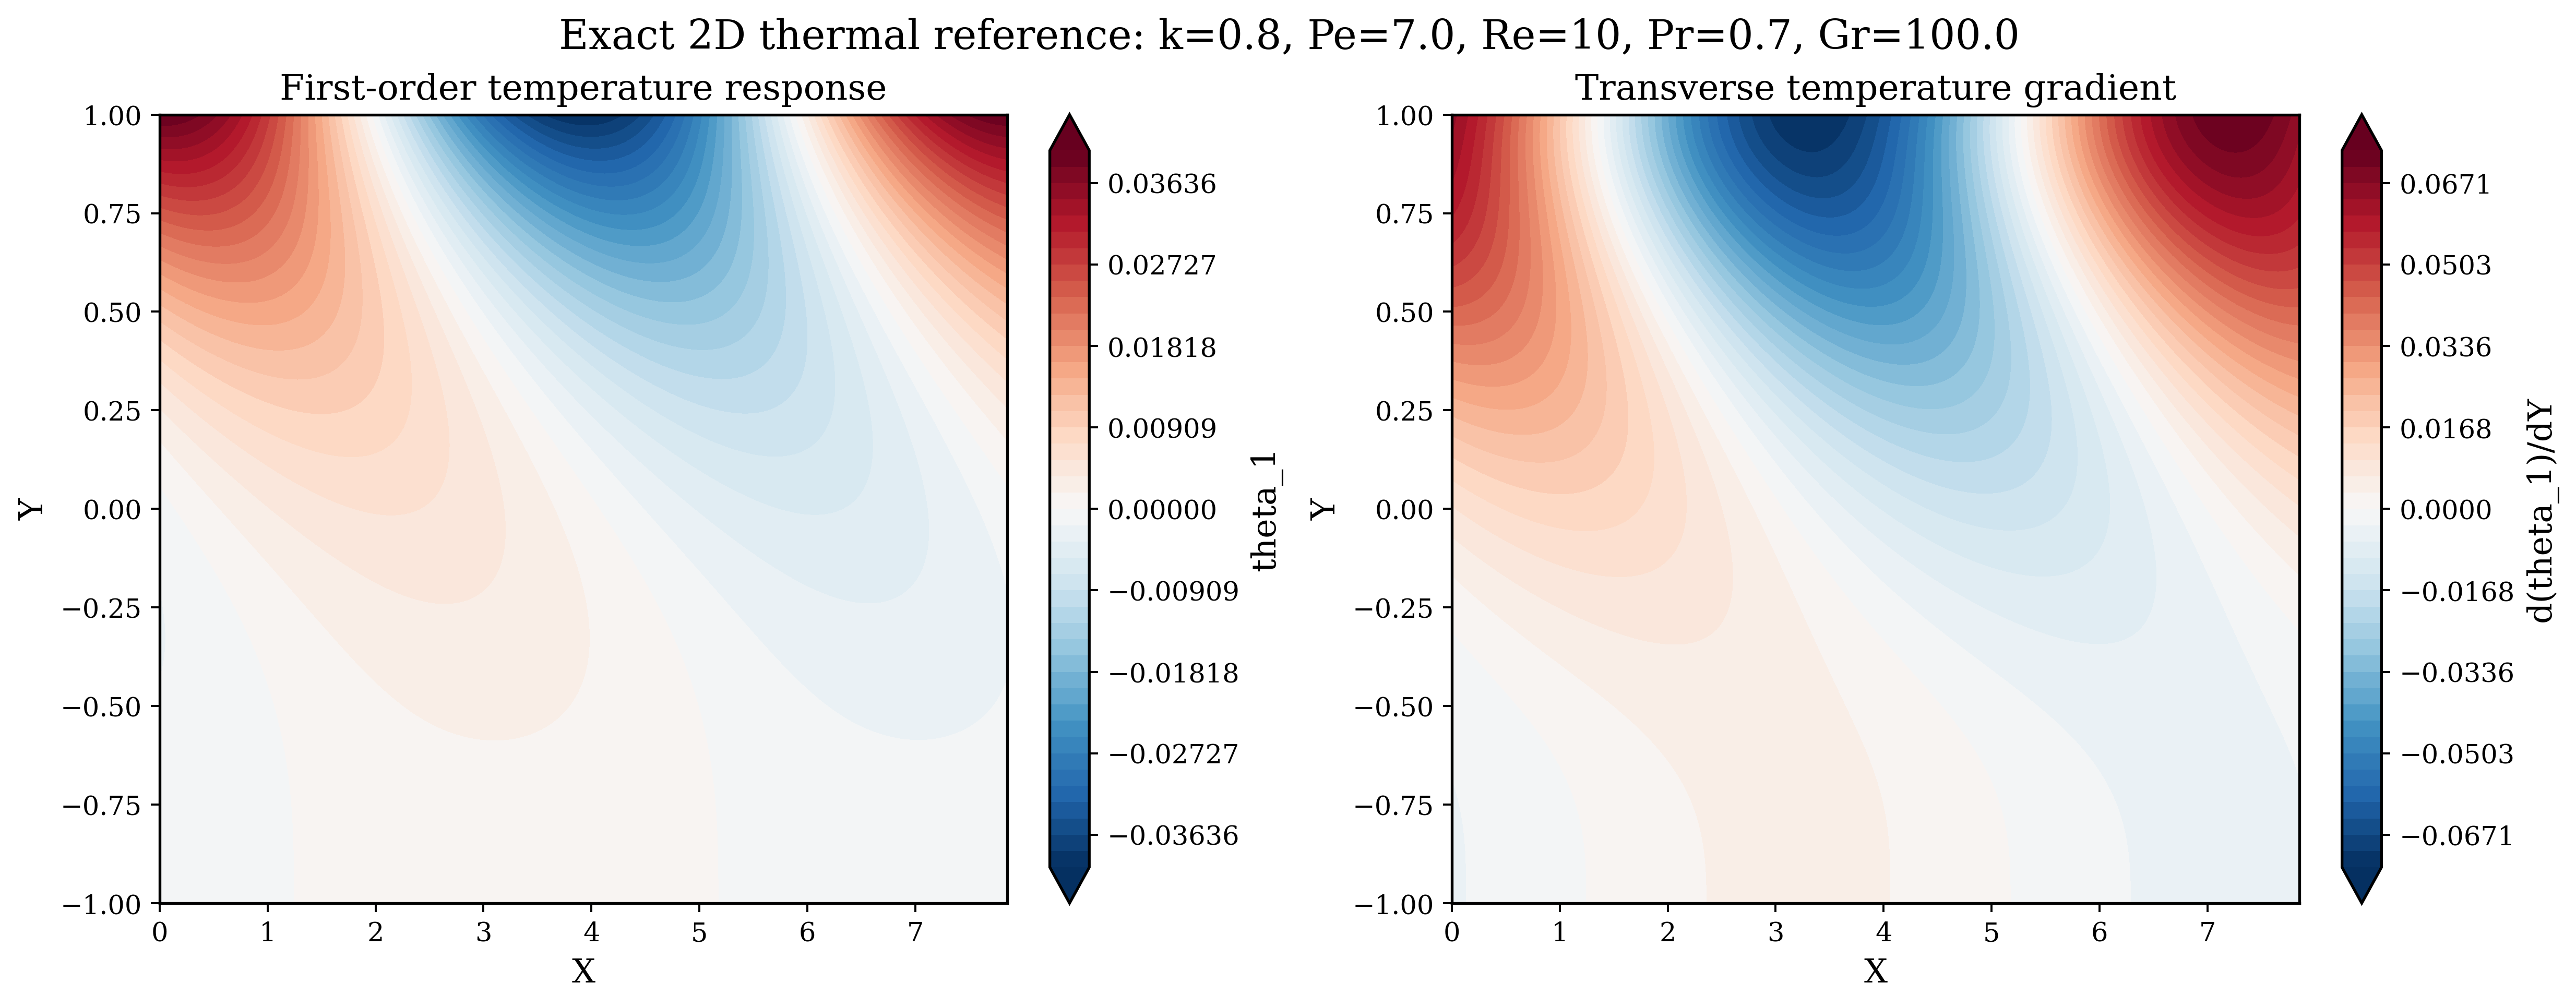
\includegraphics[width=0.90\textwidth]{fig01_temperature_reference.png}
  \caption{Two-dimensional thermal reference solution for
  $(k,\Pe,\Rey,\Pr,\Grr)=(0.8,7,10,0.7,100)$. Left: first-order temperature
  response $\theta_1(X,Y)$. Right: transverse gradient
  $\partial_Y\theta_1$, which provides the leading buoyancy forcing of the
  hydrodynamic perturbation through Eq.~\eqref{eq:V_ode}.}
  \label{fig:physical_temperature}
\end{figure}
\begin{figure}[htb]
  \centering
  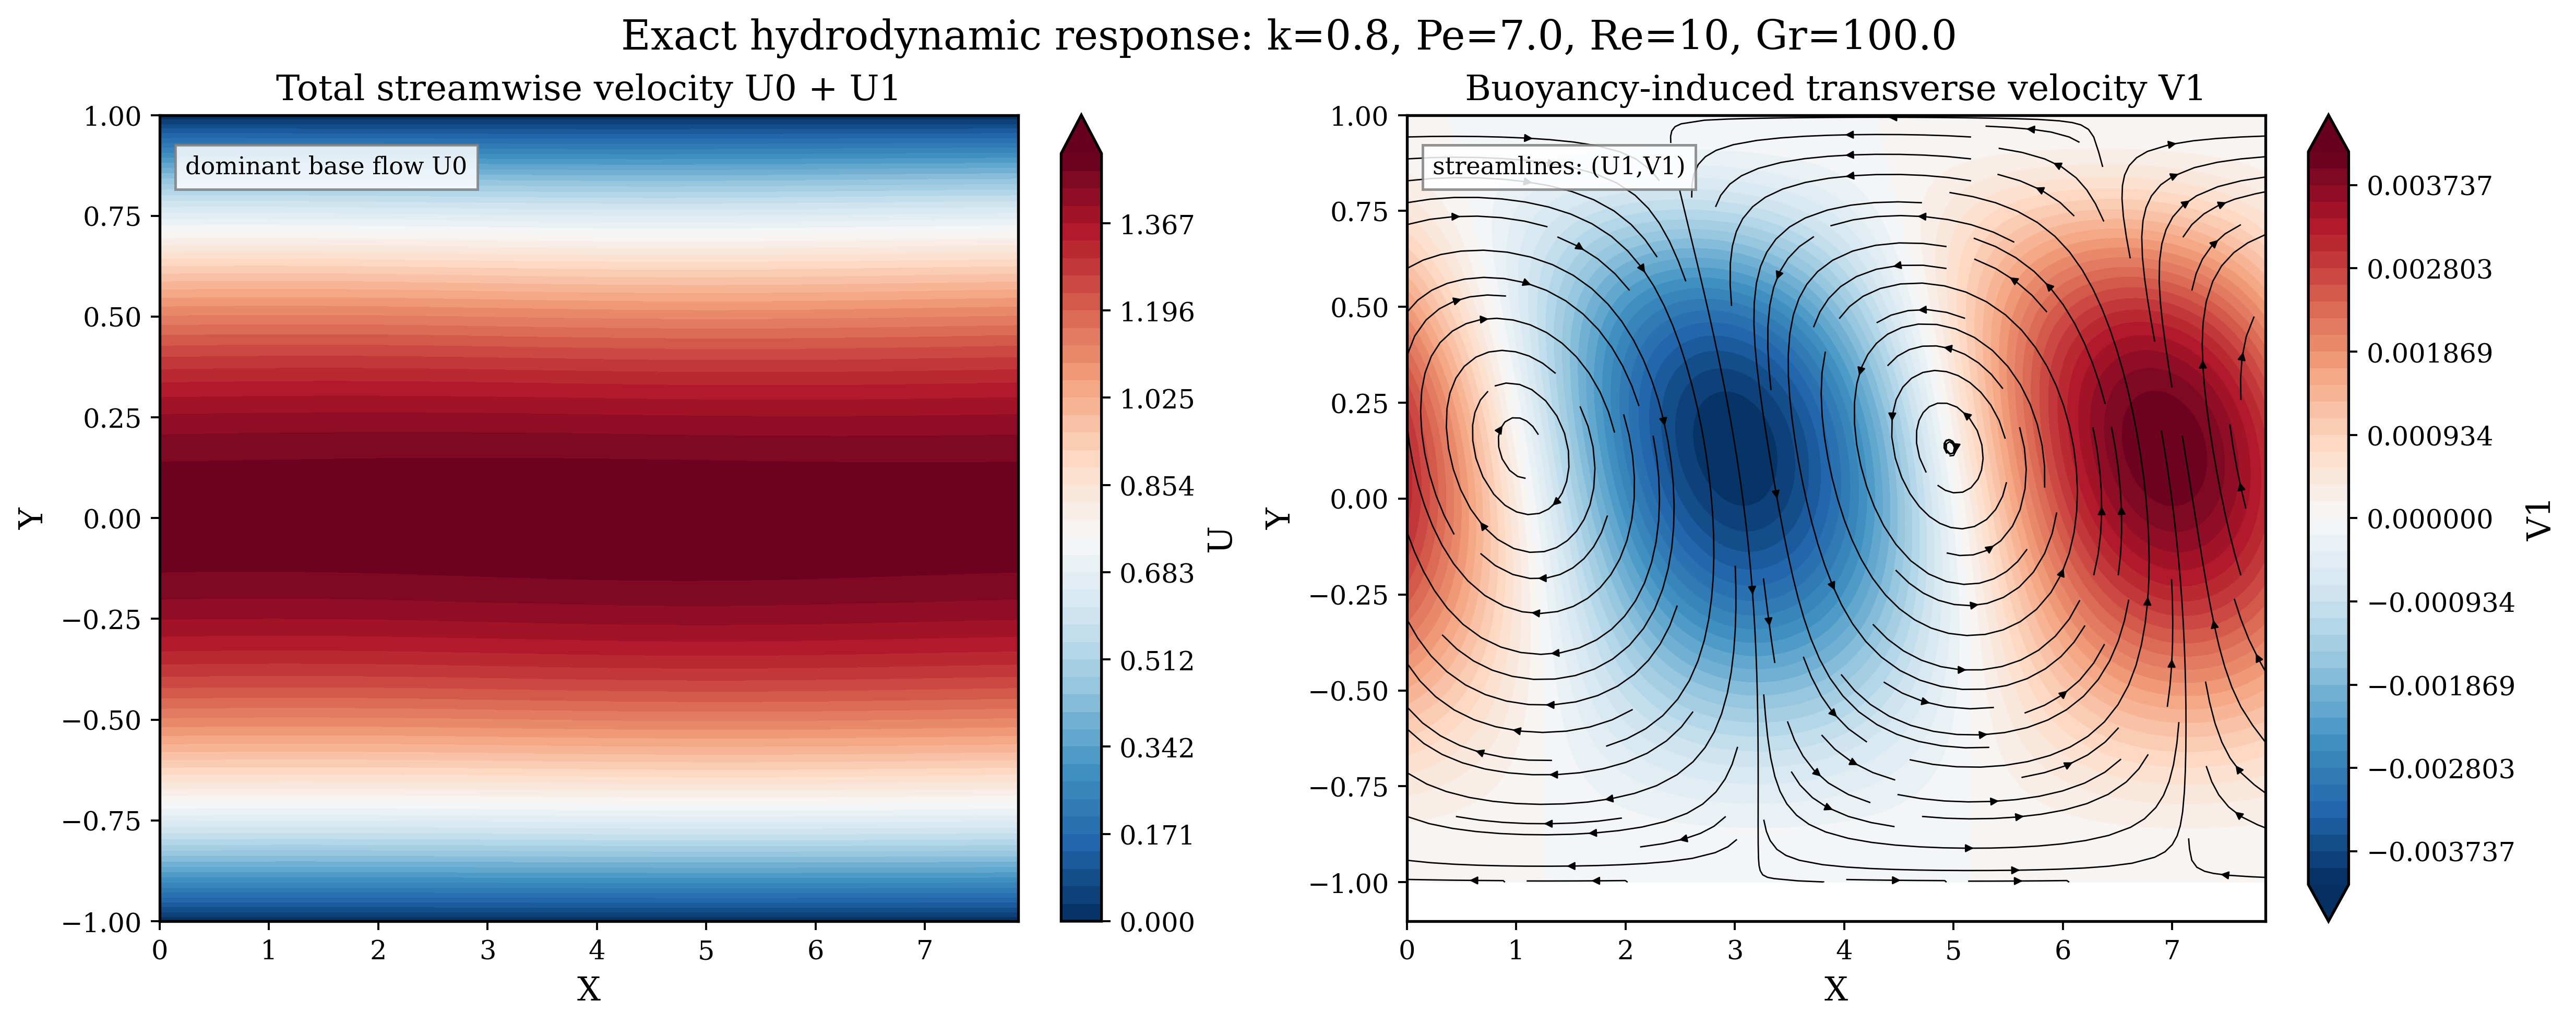
\includegraphics[width=0.90\textwidth]
  {fig02_hydrodynamic_reference.png}
  \caption{Hydrodynamic response for the reference case
  $(k,\Pe,\Rey,\Pr,\Grr)=(0.8,7,10,0.7,100)$. Left: total streamwise velocity
  $U_0+U_1$, showing the dominance of the Poiseuille base state. Right:
  buoyancy-induced transverse velocity $V_1$ with streamlines of the
  perturbation field $(U_1,V_1)$. The secondary circulation, although small
  in amplitude, is the hydrodynamic carrier of the nonlinear thermal
  redistribution.}
  \label{fig:physical_hydrodynamics}
\end{figure}
\begin{figure}[htb]
  \centering
  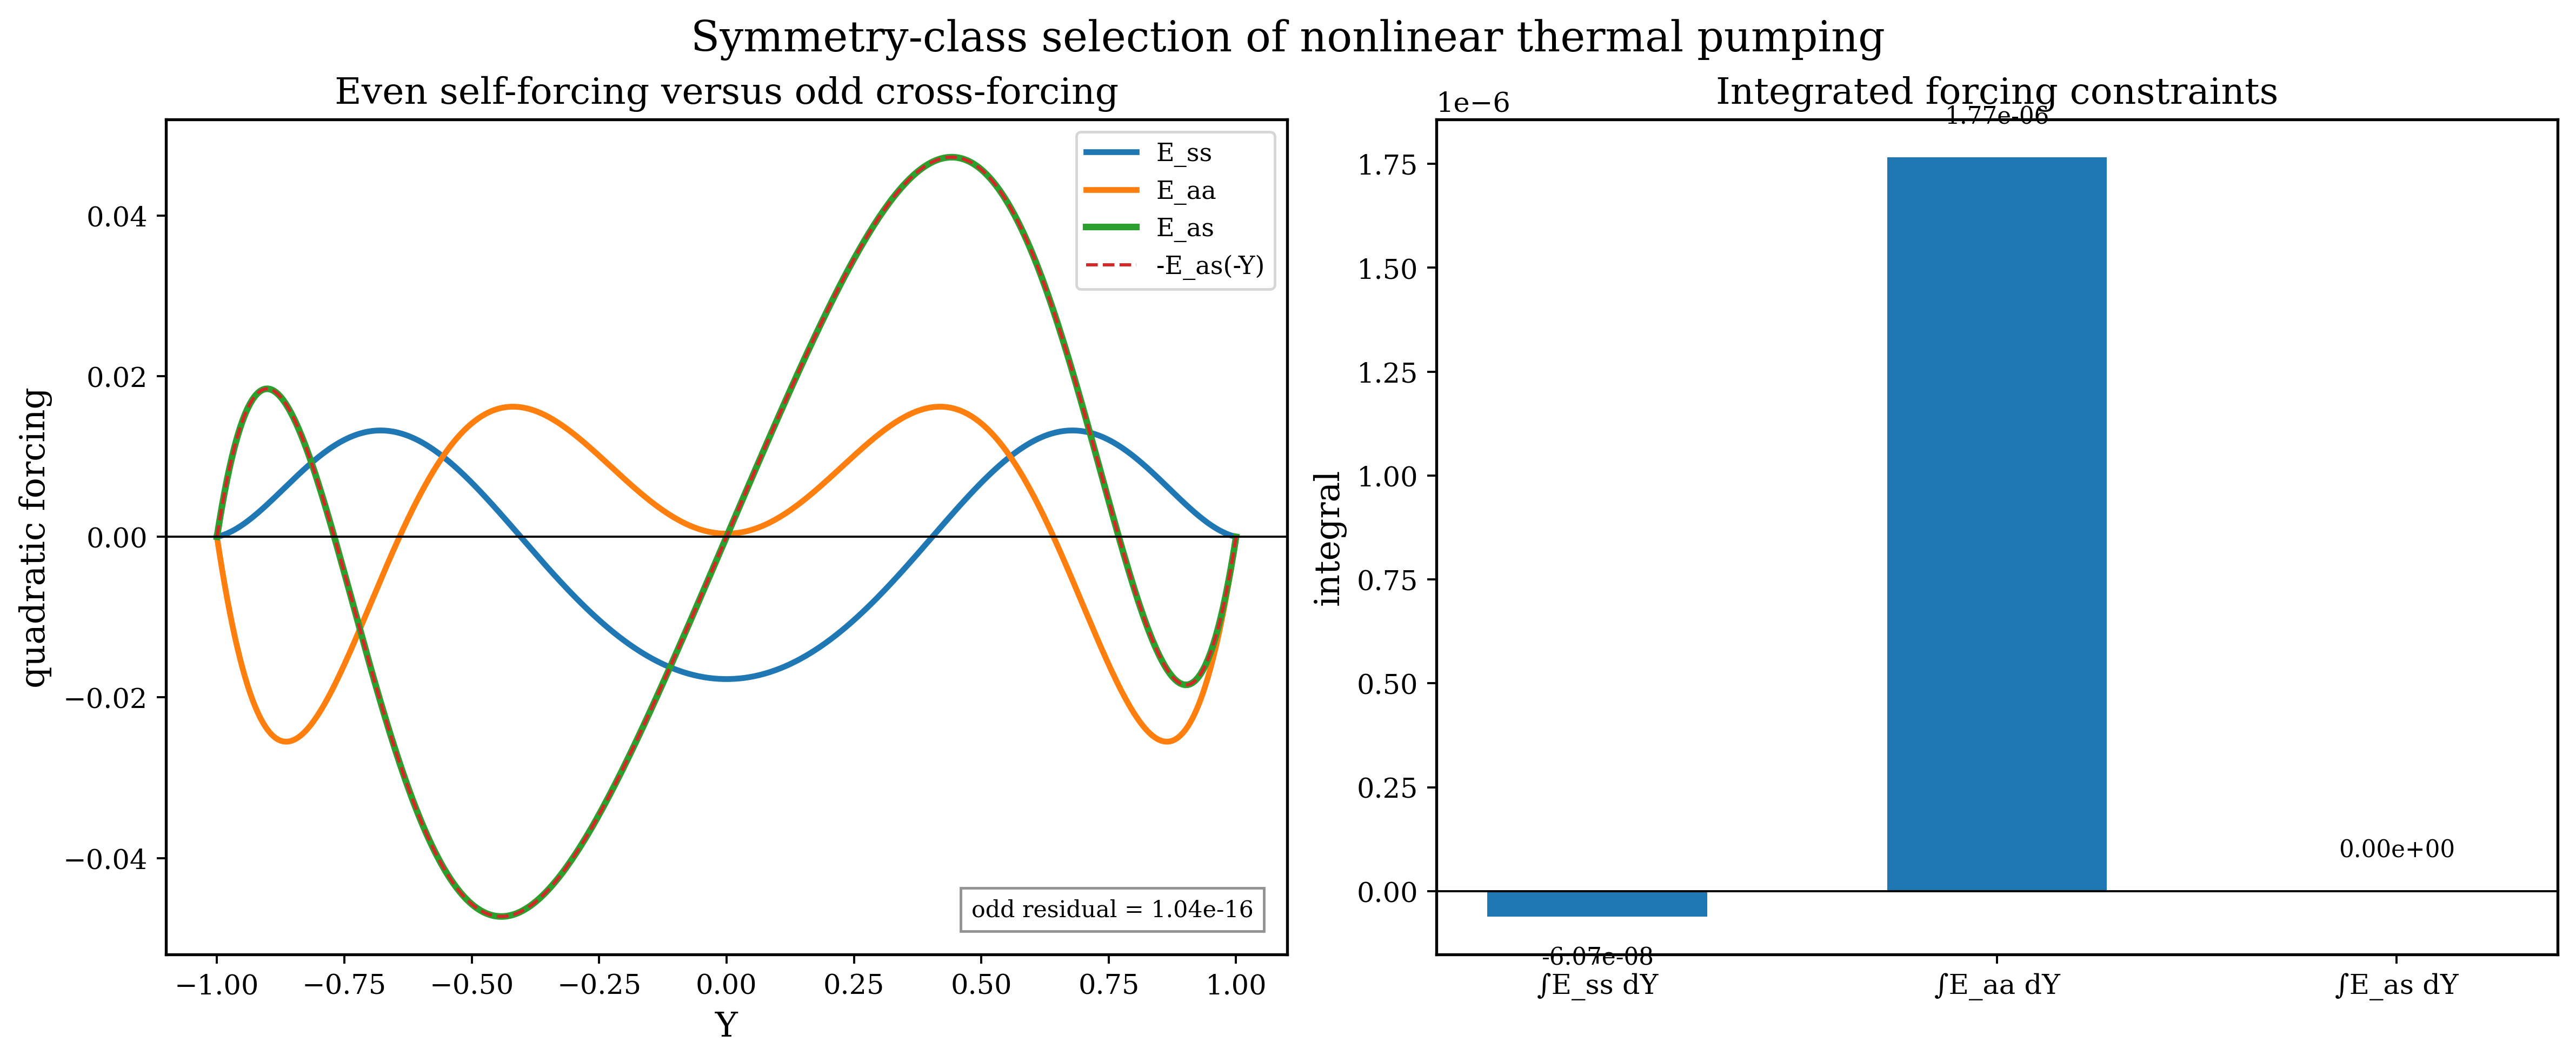
\includegraphics[width=0.90\textwidth]
  {fig04_symmetry_cross_forcing.png}
  \caption{Symmetry classification of the quadratic thermal forcing for the
  reference configuration. Left: symmetric self-interactions
  $\mathcal{E}_{ss}$ and $\mathcal{E}_{aa}$ and mixed interaction
  $\mathcal{E}_{as}$. The latter satisfies
  $\mathcal{E}_{as}(-Y)=-\mathcal{E}_{as}(Y)$, with the displayed numerical
  parity residual of order $10^{-16}$. Right: integrated forcing constraints.
  In particular, the mixed contribution has vanishing net integral, as
  required by its odd parity.}
  \label{fig:symmetry_forcing}
\end{figure}
\begin{figure}[htb]
  \centering
  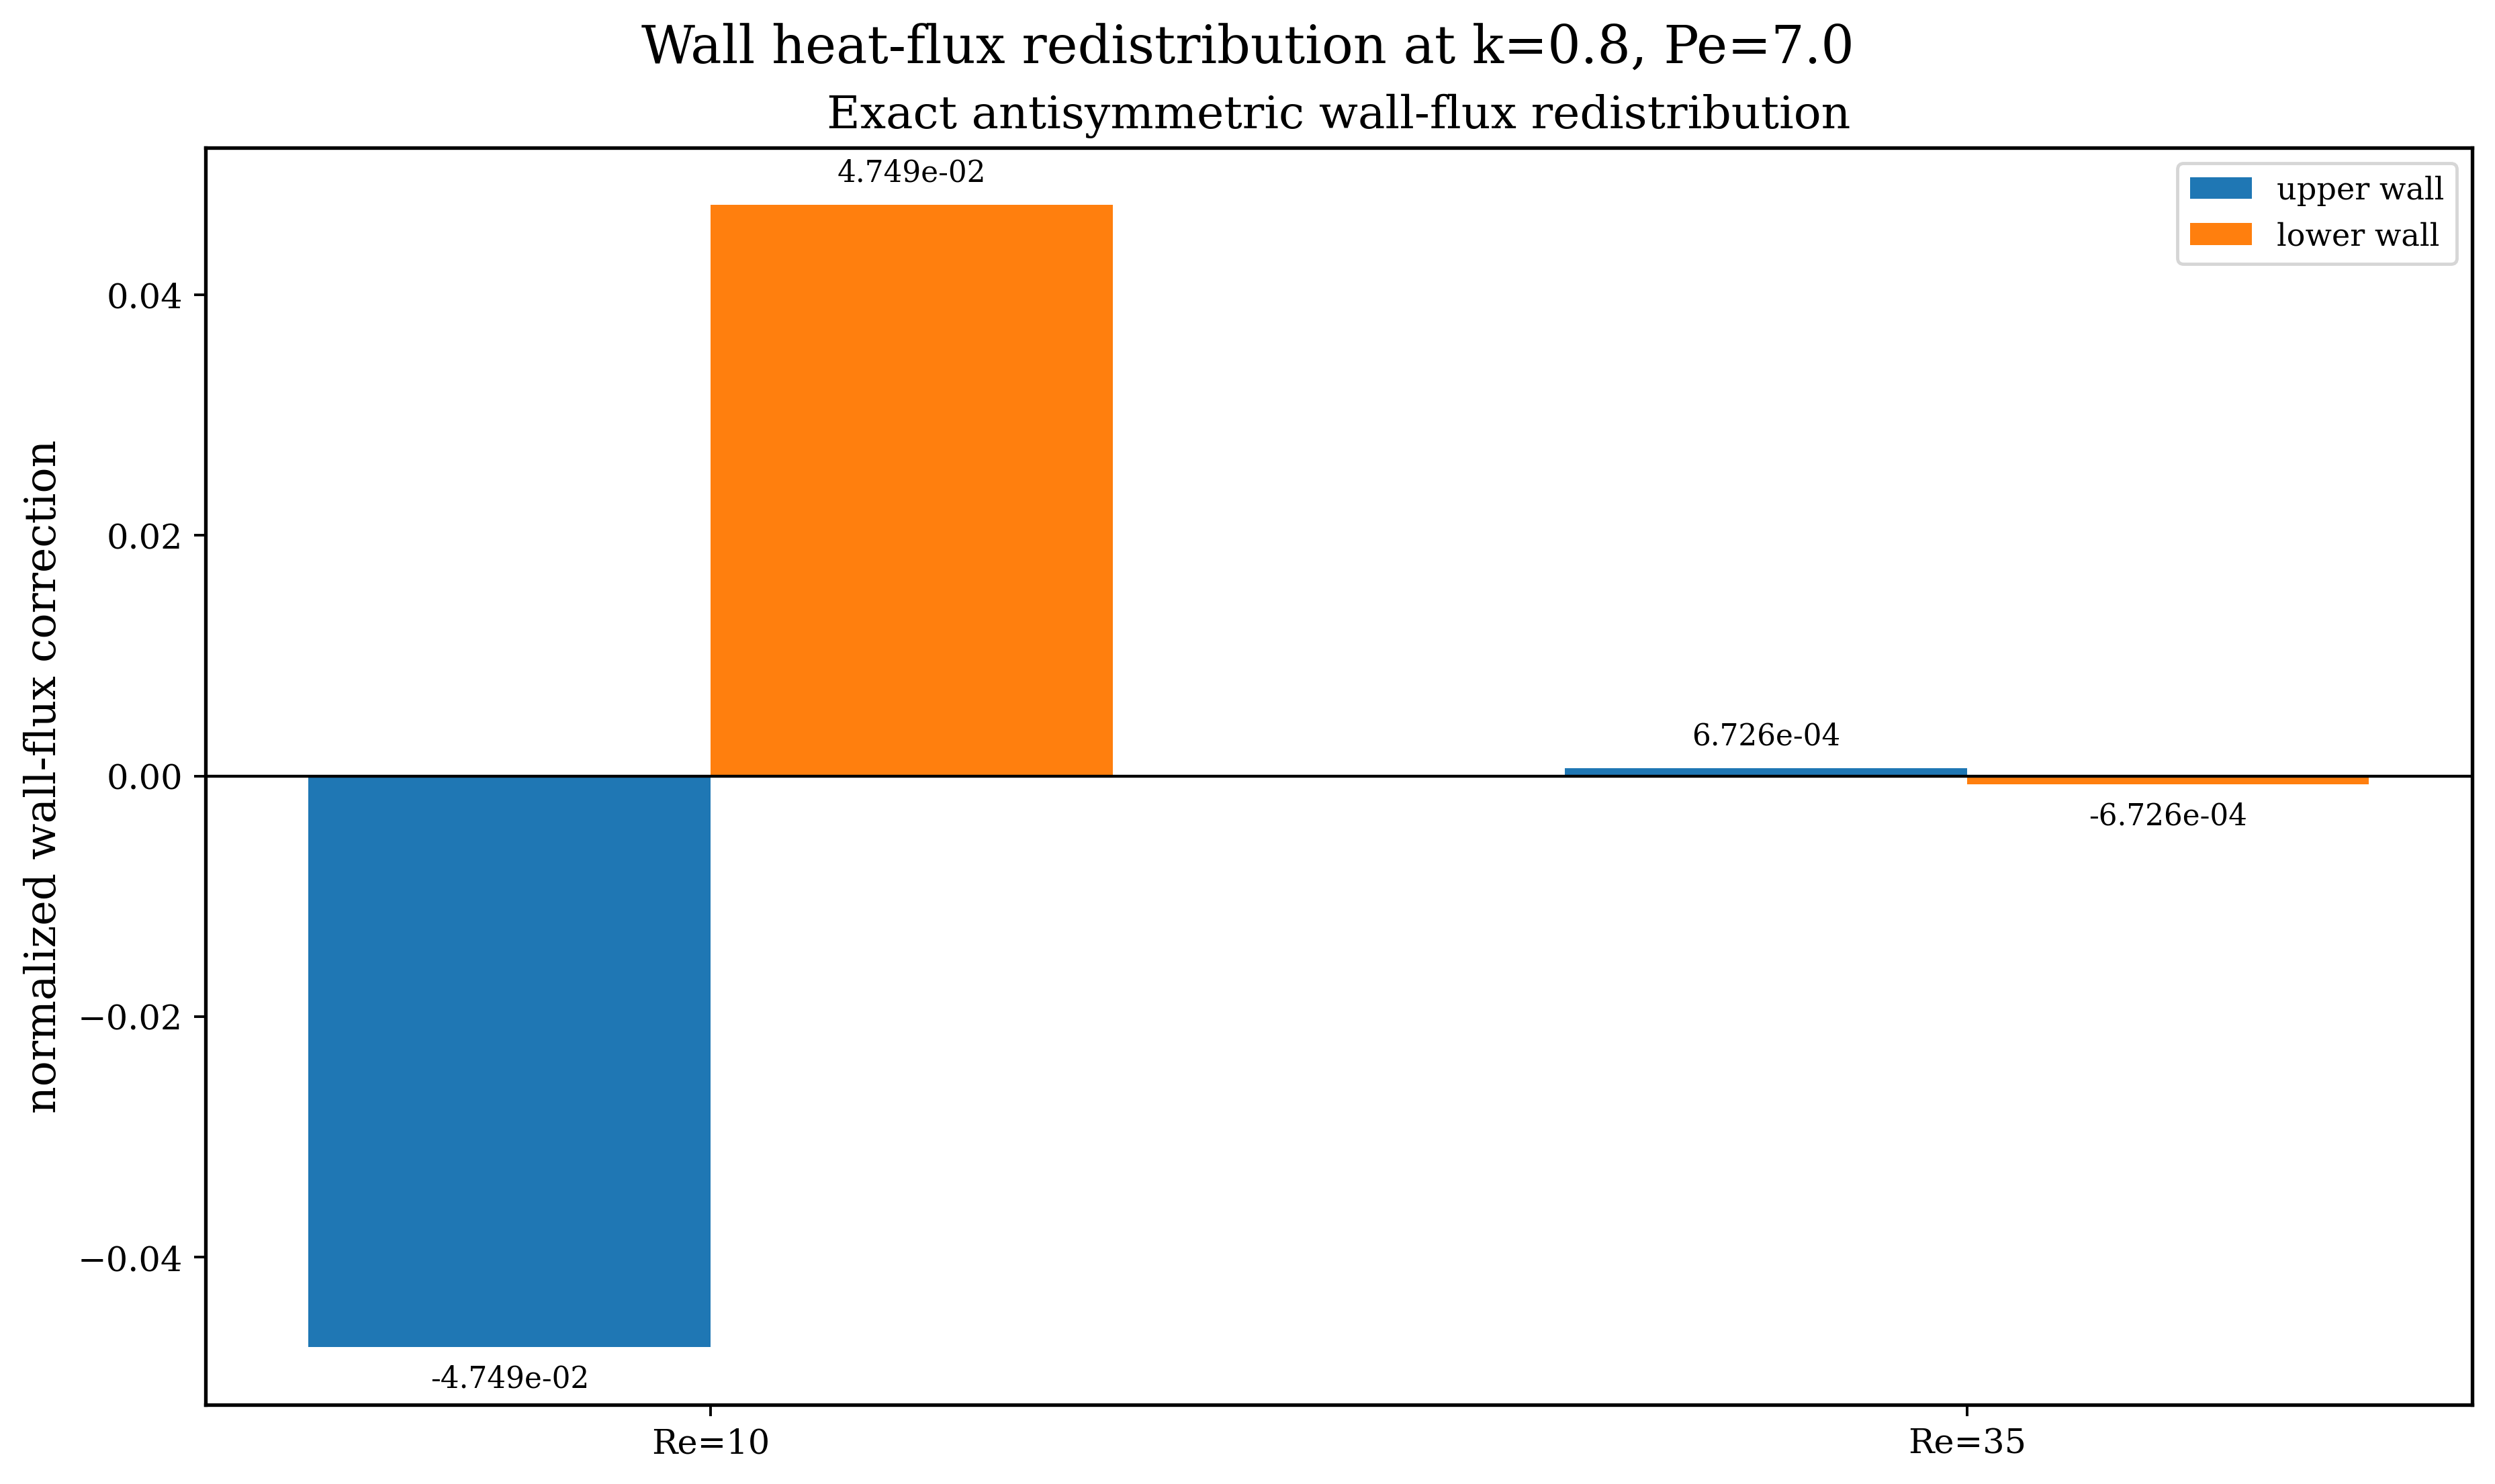
\includegraphics[width=0.76\textwidth]
  {fig03_wall_flux_redistribution.png}
  \caption{Mean nonlinear wall-flux redistribution for
  $k=0.8$ and $\Pe=7$. The comparison is performed at fixed $\Pe=7$, with
  $\Pr=\Pe/\Rey$ adjusted accordingly. The upper and lower wall corrections are equal in
  magnitude and opposite in sign, in agreement with the exact relation
  $\Nu_{2,0}(+1)=-\Nu_{2,0}(-1)$. At $\Rey=10$ the redistribution is
  comparatively strong and corresponds to $\PiT<0$, whereas at $\Rey=35$
  the amplitude is much smaller and the sign has reversed.}
  \label{fig:wall_flux_physical}
\end{figure}

\clearpage
\section{Derivations and independent checks}
\subsection{Derivation of the first-order hydrodynamic BVP}
\label{app:hydro_derivation}

For the $e^{-ikX}$ convention, incompressibility gives
$-ik\widehat U+\widehat V'=0$, hence $\widehat U=-i\widehat V'/k$. The complex perturbation vorticity is
\begin{equation}
  \widehat\omega=\partial_X\widehat V-\partial_Y\widehat U
  =\frac{i}{k}(D^2-k^2)\widehat V.
\end{equation}
Taking the streamwise derivative of the transverse momentum equation minus the transverse derivative of the
streamwise momentum equation yields
\begin{equation}
  U_0\partial_X\omega_1-V_1U_0''
  =\frac{1}{\Rey}\nabla^2\omega_1
  -\frac{\Grr}{\Rey^2}\partial_Y\theta_1.
\end{equation}
Substitution of the modal representation gives Eq.~\eqref{eq:V_ode}. The no-slip conditions imply
$\widehat V(\pm1)=\widehat V'(\pm1)=0$.

\subsection{Reflection-operator proof}
\label{app:reflection}

Define $\mathcal R[f](Y)=f(-Y)$. Since $\mathcal RD=-D\mathcal R$, $\mathcal RD^2=D^2\mathcal R$, and
$U_0,U_0''$ are even,
\begin{equation}
  \mathcal R\mathcal L_T=\mathcal L_T\mathcal R,
  \qquad
  \mathcal R\mathcal L_H=\mathcal L_H\mathcal R,
\end{equation}
where $\mathcal L_T$ and $\mathcal L_H$ denote the thermal and hydrodynamic operators. Uniqueness of
the corresponding BVPs therefore fixes the parity classes of all first-order modal fields.

\subsection{Proof of the odd cross-interaction}
\label{app:cross_proof}

Using Eq.~\eqref{eq:E_cross_complex}, the four terms have parity
\begin{align}
\widehat U^{(a)}\overline{-ik\Theta^{(s)}} &: \text{odd},\\
\widehat U^{(s)}\overline{-ik\Theta^{(a)}} &: \text{odd},\\
\widehat V^{(a)}\overline{(\Theta^{(s)})'} &: \text{odd},\\
\widehat V^{(s)}\overline{(\Theta^{(a)})'} &: \text{odd}.
\end{align}
Therefore $\mathcal E_{as}$ is odd and its channel integral vanishes.

\subsection{Mean momentum balance and fixed-bulk-flow constraint}
\label{app:mean_momentum}

The mean second-order momentum equation is
\begin{equation}
  \frac{1}{\Rey}U_{2,0}''+G_2
  =\left\langle U_1\partial_XU_1+V_1\partial_YU_1\right\rangle_X
  -\frac{\Grr}{\Rey^2}\theta_{2,0}.
\end{equation}
The conditions $U_{2,0}(\pm1)=0$ and $\int_{-1}^{1}U_{2,0}\,dY=0$ determine $G_2$ under the fixed-bulk-flow formulation.
This streaming problem is not required for the proof of wall-flux antisymmetry, but it is needed for the reported
mean-flow validation.

\subsection{Proof of the nonlinear thermal-pumping theorem}
\label{app:theorem_proof}

From
\begin{equation}
  \theta_{as,2}''=\Pe\mathcal E_{as},\qquad \theta_{as,2}(\pm1)=0,
\end{equation}
and oddness of $\mathcal E_{as}$, the function $-\theta_{as,2}(-Y)$ satisfies the same BVP as
$\theta_{as,2}$. Uniqueness gives $\theta_{as,2}(-Y)=-\theta_{as,2}(Y)$ and thus an even derivative.
The inward-normal definition of the two wall fluxes then immediately yields
$\Nu_{2,0}(+1)=-\Nu_{2,0}(-1)$.

\subsection{Proof of linearity in Grashof number}
\label{app:prop_proof}

The thermal modes are independent of $\Grr$, while the hydrodynamic BVP is linear with forcing proportional to
$\Grr\Theta'$. Consequently $\widehat V,\widehat U,\mathcal E_{as}$ and $\PiT$ are each proportional to $\Grr$ at fixed $(k,\Rey,\Pr)$.

\subsection{Integral representation of the pumping coefficient}
\label{app:mean_solution}

For $\theta''=f(Y)$ with $\theta(\pm1)=0$,
\begin{equation}
  \theta'(1)=\frac12\int_{-1}^{1}(1+Y)f(Y)\,dY,
  \qquad
  \theta'(-1)=-\frac12\int_{-1}^{1}(1-Y)f(Y)\,dY.
\end{equation}
For odd $f=\Pe\mathcal E_{as}$,
\begin{equation}
  \theta'(1)=\theta'(-1)=\frac{\Pe}{2}\int_{-1}^{1}Y\mathcal E_{as}(Y)\,dY,
\end{equation}
and the inward-normal definition gives Eq.~\eqref{eq:PiT_integral}.

\subsection{Independent validation by initial-value shooting}
\label{app:validation}

For the thermal BVP, the unknown complex derivative at $Y=-1$ is adjusted to satisfy the prescribed
value at $Y=+1$. For the fourth-order hydrodynamic BVP, the two complex initial derivatives
$\widehat V''(-1)$ and $\widehat V'''(-1)$ are adjusted until $\widehat V(+1)=\widehat V'(+1)=0$.
The shooting solutions are compared against the adaptive collocation solutions, and $\PiT$ is independently
reconstructed from the first-order fields.

%--------------------------------------------------------------
% Bibliography (single style already declared in the preamble)
% ---- Construction of the two independent mixed kernels ----
\label{sec:kernels}
\section{Construction of the two independent mixed kernels}

Let $\Theta^{(s)},\Theta^{(a)}$ denote the unit-amplitude first-order thermal modes and
$\widehat U^{(s)},\widehat V^{(s)},\widehat U^{(a)},\widehat V^{(a)}$ the corresponding
hydrodynamic modes. Their bilinear combinations fix the two real profiles that carry the
rectified response. Define
\begin{equation}
  Z_1=\widehat V^{(a)}\big(\partial_Y\Theta^{(s)}\big)^{*}
      +\widehat U^{(a)}\big(-ik\Theta^{(s)}\big)^{*},\qquad
  Z_2=\widehat V^{(s)}\big(\partial_Y\Theta^{(a)}\big)^{*}
      +\widehat U^{(s)}\big(-ik\Theta^{(a)}\big)^{*},
  \label{eq:Z_def}
\end{equation}
and, from them, the two independent mixed kernels
\begin{equation}
  \mathcal K_c=\tfrac12\Re(Z_1+Z_2),\qquad
  \mathcal K_q=\tfrac12\operatorname{Im}(Z_2-Z_1).
  \label{eq:kernels}
\end{equation}
The parity argument of Theorem~\ref{thm:symmetry} applies to \emph{each} kernel
separately: both $\mathcal K_c$ and $\mathcal K_q$ are odd in $Y$, so each produces an
odd mean temperature correction and wall-flux corrections that are equal and opposite.
The in-phase kernel $\mathcal K_c$ is the one already used in the amplitude-asymmetric
configuration, for which $d=0$; the quadrature kernel $\mathcal K_q$ is the additional
degree of freedom that phase-shifted forcing excites. Substituting
\eqref{eq:kernels} into the streamwise-averaged mixed forcing gives
Eq.~\eqref{eq:mixed_forcing_two} of the main manuscript, where the two pumping
coefficients $\PiT$ and $\PiT^{\perp}$, the exact phase law and its equal-amplitude
corollary are stated and proved.

% ---- Physical realization of the symmetry-selected mechanism ----
\section{Physical realization of the symmetry-selected pumping mechanism}
\label{sec:physical_mechanism}
%=======================================================================

The exact analysis above identifies the symmetry class of the nonlinear
wall-flux redistribution, but the corresponding physical transport pathway
is most clearly understood from the resolved two-dimensional reference
solution. We therefore consider the representative parameter set
\begin{equation}
(k,\Pe,\Rey,\Pr,\Grr)=(0.8,7,10,0.7,100),
\label{eq:physical_reference_case}
\end{equation}
which lies well inside the finite parameter domain investigated in the present
study. The wavelength is neither in the asymptotic long-wave limit nor in the
short-wave regime, while the buoyancy forcing is sufficiently strong for the
secondary hydrodynamic response to be clearly resolved. This case is used
throughout this section as a physical reference state.

A central point of the present interpretation is that the nonlinear pumping
cannot be inferred from the total velocity field alone. The base Poiseuille
flow remains dominant, whereas the buoyancy-induced perturbation is much
smaller in amplitude but is responsible for the transverse transport that
enters the quadratic thermal interaction. The reference solution therefore
provides a direct physical realization of the analytical sequence
\begin{equation}
\theta_1
\;\longrightarrow\;
\partial_Y\theta_1
\;\longrightarrow\;
(U_1,V_1)
\;\longrightarrow\;
\mathcal{E}_{as}
\;\longrightarrow\;
\PiT .
\end{equation}

%-----------------------------------------------------------------------
\subsection{Two-dimensional thermal structure and buoyancy-induced
secondary motion}
\label{subsec:2d_reference}
%-----------------------------------------------------------------------

Figure~\ref{fig:physical_temperature} shows the first-order temperature
response for the reference configuration together with its transverse
gradient. The temperature field exhibits the imposed streamwise periodicity,
while the transverse gradient is strongly structured across the channel.
This distinction is important because the buoyancy term in the linearized
momentum equation is proportional to $\Theta'(Y)$, rather than to the
temperature amplitude itself. The resolved temperature field therefore
provides the spatial structure of the thermal forcing that is subsequently
converted into a hydrodynamic response.

The corresponding hydrodynamic response is shown in
Fig.~\ref{fig:physical_hydrodynamics}. The total streamwise velocity remains
close to the Poiseuille reference profile,
\begin{equation}
U_0(Y)=\frac{3}{2}(1-Y^2),
\end{equation}
which confirms that the perturbation is a weak correction to the underlying
forced flow. In the reference calculation,
\begin{equation}
\frac{\max |U_1|}{\max |U_0|}
\simeq 6.35\times10^{-3},
\label{eq:U1_U0_ratio}
\end{equation}
whereas the transverse velocity is of the same order as the perturbation
streamwise velocity and is therefore dynamically relevant even though both
remain small compared with the base flow.

For this reason, the streamlines shown in the right panel of
Fig.~\ref{fig:physical_hydrodynamics} are constructed from the perturbation
field $(U_1,V_1)$ rather than from the total velocity $(U_0+U_1,V_1)$.
The latter would be overwhelmingly dominated by the nearly parallel
Poiseuille component and would obscure the secondary transport. The
perturbation streamlines reveal a streamwise-periodic secondary circulation
induced by buoyancy. These secondary motions provide the transverse advection
required to convert the imposed thermal modulation into a nonzero quadratic
mean response.

The reference solution therefore gives a useful physical interpretation of
the analytical scaling
\begin{equation}
\widehat V^{(j)}\propto\Grr.
\end{equation}
Buoyancy does not alter the first-order thermal modes at fixed $(k,\Pe)$;
instead, it provides the hydrodynamic mediator through which the thermal
asymmetry is converted into a transverse transport process. This is also
consistent with the exact switch-off result $\PiT=0$ at $\Grr=0$. The profile-level signature of
that odd response, for a strongly asymmetric wall forcing, is shown in Fig.~\ref{fig:profiles}.

\begin{figure}[htb]
  \centering
  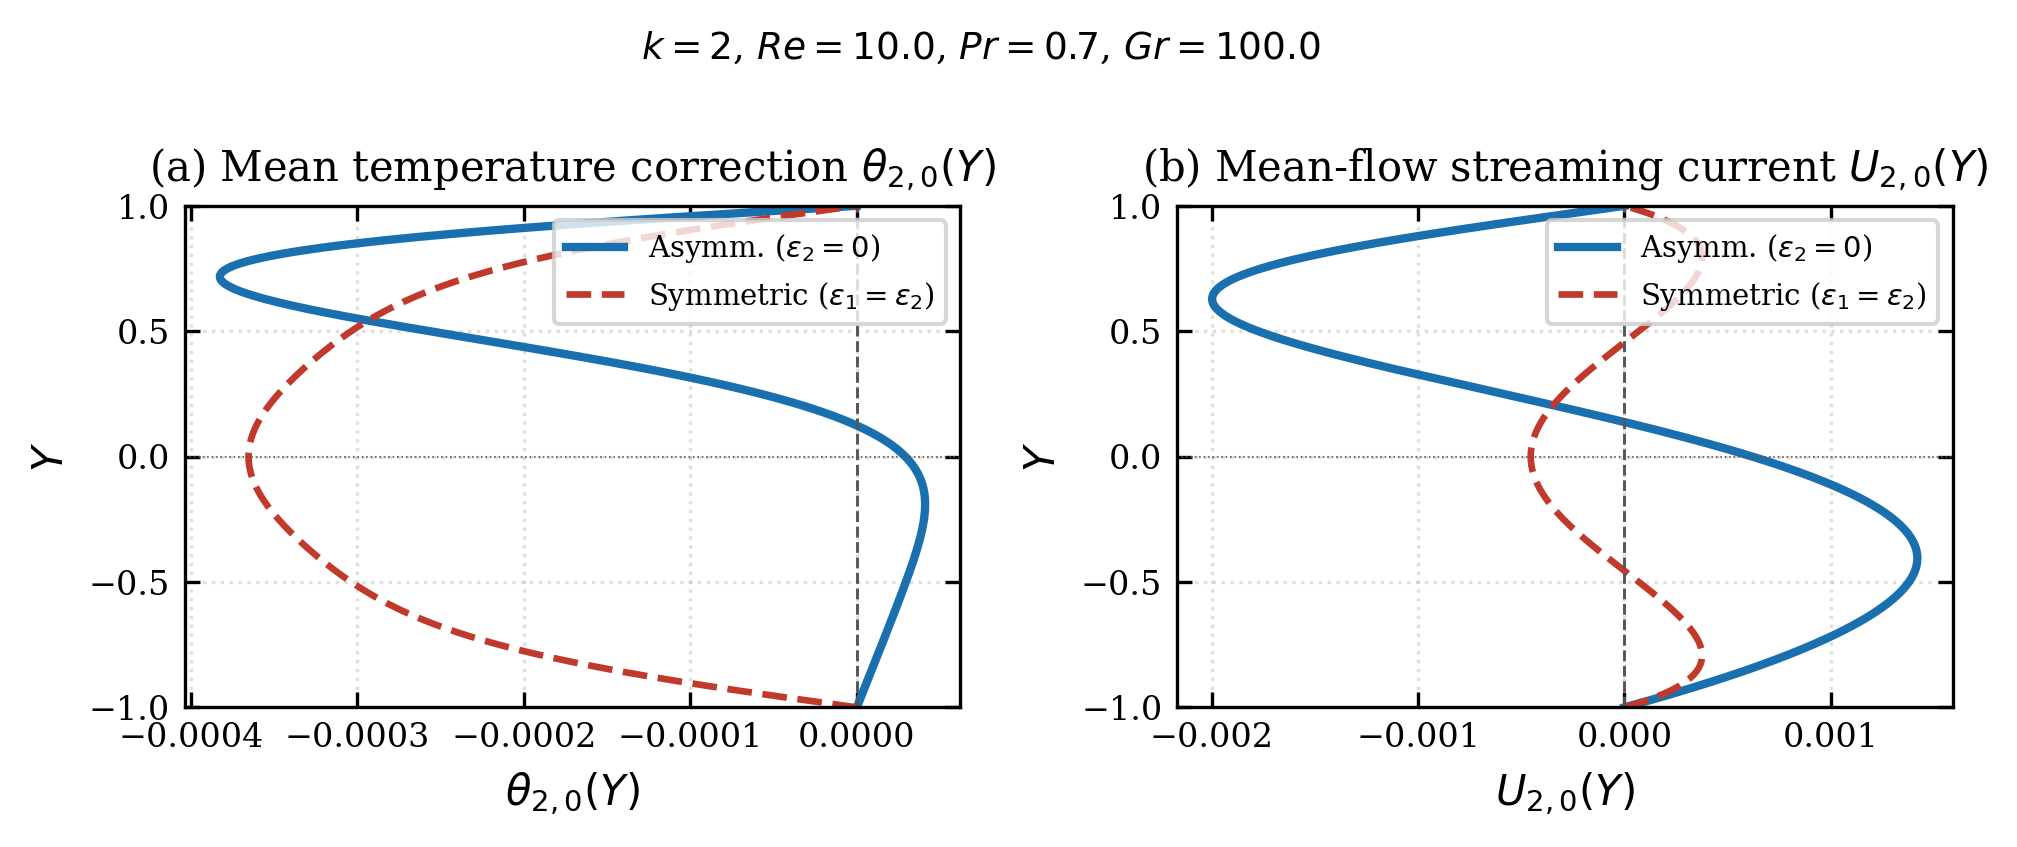
\includegraphics[width=0.90\textwidth]{fig02_profiles.png}
  \caption{Cross-channel profiles of the mean temperature correction $\theta_{2,0}(Y)$ and the mean
  streaming velocity $U_{2,0}(Y)$ for a strongly asymmetric wall forcing. The odd thermal profile is the
  direct profile-level manifestation of the analytical symmetry theorem.}
  \label{fig:profiles}
\end{figure}

%-----------------------------------------------------------------------
\subsection{Symmetry selection of the nonlinear interaction}
\label{subsec:symmetry_selection_physical}
%-----------------------------------------------------------------------

The next step is to identify which part of the quadratic interaction is
capable of producing a net wall-flux redistribution. Figure~\ref{fig:symmetry_forcing}
shows the three quadratic forcing classes appearing in the streamwise-mean
thermal equation. The self-interactions,
$\mathcal{E}_{ss}$ and $\mathcal{E}_{aa}$, belong to the even symmetry class,
whereas the mixed interaction $\mathcal{E}_{as}$ is odd under the reflection
$Y\rightarrow -Y$.

The numerical structure shown in Fig.~\ref{fig:symmetry_forcing} provides a
direct physical counterpart to the operator-based parity proof. The relevant
observation is not simply that $\mathcal{E}_{as}$ changes sign across the
channel, but that its positive and negative regions are organized in such a
way that their unweighted integral cancels. Consequently, the mixed
interaction does not act as a net volumetric heat source. Instead, it
redistributes the mean thermal response transversely.

This distinction is essential. The nonlinear pumping observable is not
controlled by the zeroth moment
\begin{equation}
\int_{-1}^{1}\mathcal{E}_{as}(Y)\,dY,
\end{equation}
which vanishes, but by its first transverse moment. From
Eq.~\eqref{eq:PiT_integral},
\begin{equation}
\PiT=
-\frac{\Pe}{2}
\int_{-1}^{1}Y\,\mathcal{E}_{as}(Y)\,dY.
\label{eq:PiT_first_moment_physical}
\end{equation}
The pumping mechanism can therefore be interpreted as a
\emph{transverse rectification} of a locally balanced nonlinear interaction:
the mixed forcing produces no net mean heat source, but its spatial
distribution with respect to the channel centerline generates a finite
redistribution of the two wall heat fluxes.

This interpretation also explains why the distinction between symmetry and
magnitude must be maintained. The odd parity of $\mathcal{E}_{as}$ is fixed
by reflection symmetry, whereas the magnitude and sign of its first moment
remain determined by the coupled thermal--hydrodynamic dynamics.

%-----------------------------------------------------------------------
\subsection{From local nonlinear interaction to wall-flux redistribution}
\label{subsec:wall_flux_rectification}
%-----------------------------------------------------------------------

The macroscopic consequence of the mixed interaction is the antisymmetric
wall-flux correction established analytically above. For the fixed-$\Pe$
Reynolds-number comparison, $\Pr$ is adjusted according to $\Pr=\Pe/\Rey$;
thus the cases $\Rey=10$ and $\Rey=35$ at $\Pe=7$ correspond to $\Pr=0.7$
and $\Pr=0.2$, respectively. For the present
reference configuration ($\Rey=10$, $\Pr=0.7$), the normalized pumping coefficient is
\begin{equation}
\PiT(\Rey=10)
=-4.7492\times10^{-2},
\end{equation}
while at the same $k$ and $\Pe$, but with $\Rey=35$ ($\Pr=0.2$),
\begin{equation}
\PiT(\Rey=35)
=6.7256\times10^{-4}.
\end{equation}
Figure~\ref{fig:wall_flux_physical} displays the corresponding upper- and
lower-wall corrections.

For $\Rey=10$, the negative value of $\PiT$ indicates that the upper-wall
correction is directed opposite to the convention adopted for positive
pumping, while the lower wall receives the compensating correction. The
important point is that the total mean wall contribution remains balanced:
the nonlinear mechanism redistributes the flux rather than creating an
additional net heat input at second order.

The contrast between $\Rey=10$ and $\Rey=35$ is particularly informative.
The first-order thermal problem depends on $\Rey$ and $\Pr$ through the
combination $\Pe=\Rey\Pr$, but the hydrodynamic response retains an explicit
dependence on $\Rey$. Consequently, keeping $\Pe$ fixed does not preserve
the nonlinear pumping response. The two cases therefore provide a direct
physical demonstration of the parameter-dependence argument developed in
Sec.~\ref{sec:results}: Reynolds number controls the hydrodynamic realization
of the same thermal forcing.

%-----------------------------------------------------------------------
\subsection{Hydrodynamic control of pumping direction}
\label{subsec:reversal_physical}
%-----------------------------------------------------------------------

The sign reversal observed in Fig.~\ref{fig:wall_flux_physical} is the most
useful physical consequence of the coupled formulation because it goes beyond
the exact symmetry statement. At fixed $k=0.8$, $\Pe=7$ and $\Grr=100$, the
normalized pumping response changes sign between $\Rey=10$ and $\Rey=35$,
with a reversal near
\begin{equation}
\Rey_c\simeq30.84.
\label{eq:Recritical_physical}
\end{equation}

This behavior should not be interpreted as a change in the symmetry class.
The relation
\begin{equation}
\Nu_{2,0}(+1)=-\Nu_{2,0}(-1)
\end{equation}
remains valid on both sides of the crossing. What changes is the sign of the
first transverse moment in Eq.~\eqref{eq:PiT_first_moment_physical}.
Increasing $\Rey$ modifies the phase and spatial distribution of the
buoyancy-induced transverse velocity relative to the thermal field, and
therefore changes the signed overlap that enters $\mathcal{E}_{as}$.
The reversal is thus a \emph{dynamical} effect superimposed on an unchanged
symmetry constraint.

In physical terms, the imposed thermal modulation establishes the spatial
temperature pattern, buoyancy converts the transverse temperature gradient
into a secondary circulation, and the Reynolds number controls how that
circulation is phase-shifted and spatially weighted relative to the thermal
pattern. The resulting quadratic overlap can consequently transfer the
preferential wall-flux redistribution from one wall to the other without any
change in the underlying reflection symmetry.

This provides a useful distinction between two classes of results obtained in
the present study:
\begin{equation}
\boxed{
\begin{array}{ll}
\text{symmetry-controlled:}
&
\Nu_{2,0}(+1)=-\Nu_{2,0}(-1),
\\[2mm]
\text{dynamics-controlled:}
&
|\PiT|,\quad
\operatorname{sign}(\PiT),\quad
\Rey_c,\quad
k^*(\Pe).
\end{array}}
\label{eq:symmetry_vs_dynamics}
\end{equation}
The first relation is exact under the assumptions of the theory, whereas the
second set of quantities must be determined from the coupled thermal and
hydrodynamic response.

%-----------------------------------------------------------------------
\subsection{Physical picture of nonlinear thermal pumping}
\label{subsec:physical_picture}
%-----------------------------------------------------------------------

The resolved reference solution suggests a compact physical picture of the
pumping mechanism. The periodic thermal boundary condition first creates a
streamwise-organized temperature field. Its transverse gradient generates a
buoyancy force, which produces a weak but spatially structured secondary
velocity field. The interaction between the symmetric and antisymmetric
components of this response generates the odd forcing
$\mathcal{E}_{as}$. Although that forcing has zero net integral, its nonzero
first transverse moment produces a finite wall-flux difference. The nonlinear
pumping coefficient therefore measures a rectified transverse redistribution
rather than a net creation of thermal energy.

The mechanism may be summarized schematically as
\begin{equation*}
\begin{aligned}
\text{periodic thermal pattern}
&\;\xrightarrow{\;\partial_Y\theta_1\;}
\text{buoyancy-induced secondary flow} \\
&\;\xrightarrow{\;\text{quadratic interaction}\;}
\mathcal{E}_{as}(Y)
\;\xrightarrow{\;Y\text{-moment}\;}
\PiT .
\end{aligned}
\end{equation*}

This interpretation also clarifies why the pumping disappears in the
forced-convection limit $\Grr=0$. Without buoyancy, the secondary
hydrodynamic mediator vanishes and the mixed thermal interaction cannot
generate the wall-flux redistribution considered here. Conversely, when
buoyancy is present, the symmetry-breaking boundary condition determines the
admissible redistribution pattern, while the hydrodynamic parameters
determine its magnitude and direction.

A useful physical interpretation follows from the geometry of the zero set.
The disappearance of positive pumping for $\Pe>\Pe_c$ does not occur through
a loss of the symmetry-breaking mechanism itself. The odd cross-interaction
$\mathcal{E}_{as}$ remains structurally admissible, and the exact wall-flux
antisymmetry remains unchanged. Instead, the region of parameter space in
which the first transverse moment of $\mathcal{E}_{as}$ is positive contracts
toward larger wavenumbers until the zero set reaches the upper boundary
$k=10$. The post-critical regime therefore corresponds to the expulsion of
the sign-changing locus from the finite admissible domain, rather than to the
disappearance of the underlying nonlinear interaction. This interpretation
is consistent with the simultaneous preservation of the symmetry class and
the continuous local sign change observed in $\PiT(10,\Pe)$ near $\Pe_c$.

\end{document}
